\chapter{Diseño e Implementación}
\label{cap:Diseño-Implementacion}
\graphicspath{ {Imagenes/Figuras/} }

En este capítulo se presentan diferentes fases del proyecto que permiten explicar por qué utilizamos las tecnologías mencionadas y reproducir la ejecución del mismo a través de un manual de instalación y configuración.

\section{Fase de Análisis}
Una vez planteado el proyecto se analizaron diferentes tecnologías y lenguajes de programación para afrontar su implementación.
La aplicación web teníamos claro que la íbamos a desarrollar con JavaScript y HTML, ya que no teníamos experiencia previa creando páginas web y estos lenguajes son los más usados y podemos encontrar mucha información sobre ellos. Para la creación de la aplicación móvil tuvimos más dudas: empezamos intentando crear un proyecto usando Xamarin ~\citep{platzi}, puesto que Jesús tenía algo de experiencia previa con ese lenguaje, pero al poco tiempo vimos que nos daba algunos problemas, por lo que decidimos cambiar el proyecto a Android Studio. Jorge ya había usado este programa en otra asignatura, así que teníamos esa ventaja. Además, es un entorno más sencillo e intuitivo para crear aplicaciones móviles.

En cuanto a la base de datos, la primera idea era generar una base de datos relacional con MySql o con Oracle, pero debatiendo nos dimos cuenta de que para un proyecto de este tipo, en el que no se necesitaba una gran base de datos, el uso de una base de datos no relacional, como la que ofrece \textit{Firebase} nos proporcionaba más seguridad y una mejor y más sencilla implementación.

\section{Fase de Investigación}

Una vez elegidas las tecnologías a usar en la fase de análisis, nos encontramos ante algunas dificultades, como los lenguajes web y el servicio de \textit{Firebase}. Los lenguajes web no los habíamos visto prácticamente durante la carrera, al igual que las bases de datos no relacionales, así que nos pusimos a hacer algún curso online (un curso JavaScript en Platzi ~\citep{platzi} y algunos tutoriales de \textit{Firebase}) con los que poder empezar a trabajar en estos proyectos.

\section{Fase de Instalación y Configuración}
En esta sección se describen los pasos a seguir para recrear y ejecutar el proyecto.
\subsubsection*{Paso 1. Creación de un proyecto en GitHub}
Para mantener el control de versiones y copias de seguridad constantes del proyecto, se utiliza un proyecto en GitHub, y su aplicación de escritorio GitHub Desktop para manejarlo más fácilmente.


\subsubsection*{Paso 2. Instalación de Android Studio}
Se descargó la aplicación de código abierto oficial de Android para el desarrollo de la aplicación móvil.

\begin{figure}[h]
    \centering
    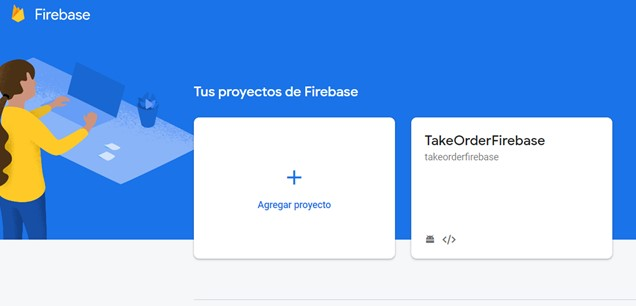
\includegraphics[width=13cm, height=7cm]{Imagenes/Figuras/FirebaseCrearProyecto.jpg} 
   \caption{Creación de un nuevo proyecto Firebase\label{fig:Firea}}
\end{figure}

\begin{figure}[h]
    \centering
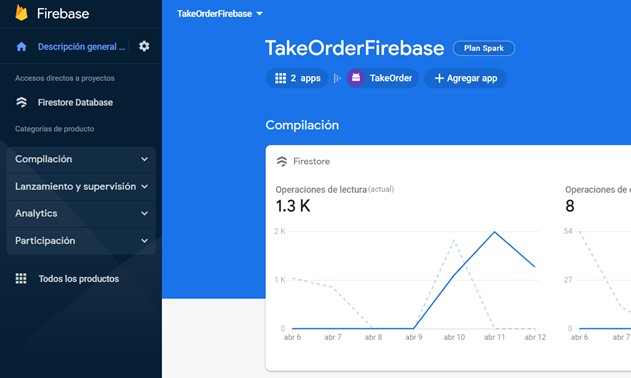
\includegraphics[width=13cm, height=7cm]{Imagenes/Figuras/FirebaseMuestraProyecto.jpg} 
   \caption{Menú inicio proyecto Firebase\label{fig:Fireb}}
\end{figure}

\subsubsection*{Paso 3. Instalación de Visual Studio Code}
Se descargó la aplicación de Visual Studio Code ~\citep{VSCode} desde su página oficial.

\subsubsection*{Paso 4. Creación de un proyecto en Firebase}

Se ha desarrollado un proyecto en \textit{Firebase} para registrar y administrar el restaurante, el cual se integrará con las aplicaciones web y móvil.

Para llevar a cabo esto, hay que acceder a la plataforma de \textit{Firebase} y autenticarse con una cuenta de Google. Una vez iniciada la sesión, creamos un proyecto nuevo (como se muestra en la Figura~\ref{fig:Firea}) y rellenamos el formulario con información como el nombre del proyecto y su ubicación.

\textit{Firebase} nos ofrece dos tipos de base de datos: \textit{Cloud Firestore} o \textit{Realtime Database}. \textit{Cloud Firestore} es la base de datos más reciente de \textit{Firebase} y mejora en muchos aspectos (consultas más ricas y rápidas, nuevo modelo de datos más intuitivo...) a la original, \textit{Realtime Database}, por lo que nos decidimos a usar esta nueva solución.

Cuando hayamos creado el proyecto llegamos a su página principal(Figura~\ref{fig:Fireb}), desde la que podremos acceder a los diferentes menús donde nos ofrecen un montón de métricas de nuestras aplicaciones que podemos consultar(Figura~\ref{fig:Analytics}).

Ya solo nos queda vincular nuestro proyecto de \textit{Firebase} con nuestras aplicaciones. Para ello tenemos que pulsar sobre el icono \textit{settings} a la derecha del nombre del proyecto, y en la pestaña general nos dará la opción de vincular nuestras aplicaciones (Figura~\ref{fig:AddApp}).



Seguiremos todos los pasos que nos va indicando \textit{Firebase}, entre los cuales está añadir un trozo de código con todos los parámetros necesarios para realizar la conexión.

Una vez finalizada la conexión de la aplicación con \textit{Firebase} podremos hacer uso de las utilidades de las que dispone, como el acceso a la base de datos de usuarios, llamada
\textit{Authentication}, y la base de datos no relacional que se encuentra en la pestaña \textit{Firestore Database}.

\begin{figure}[h]
    \centering
    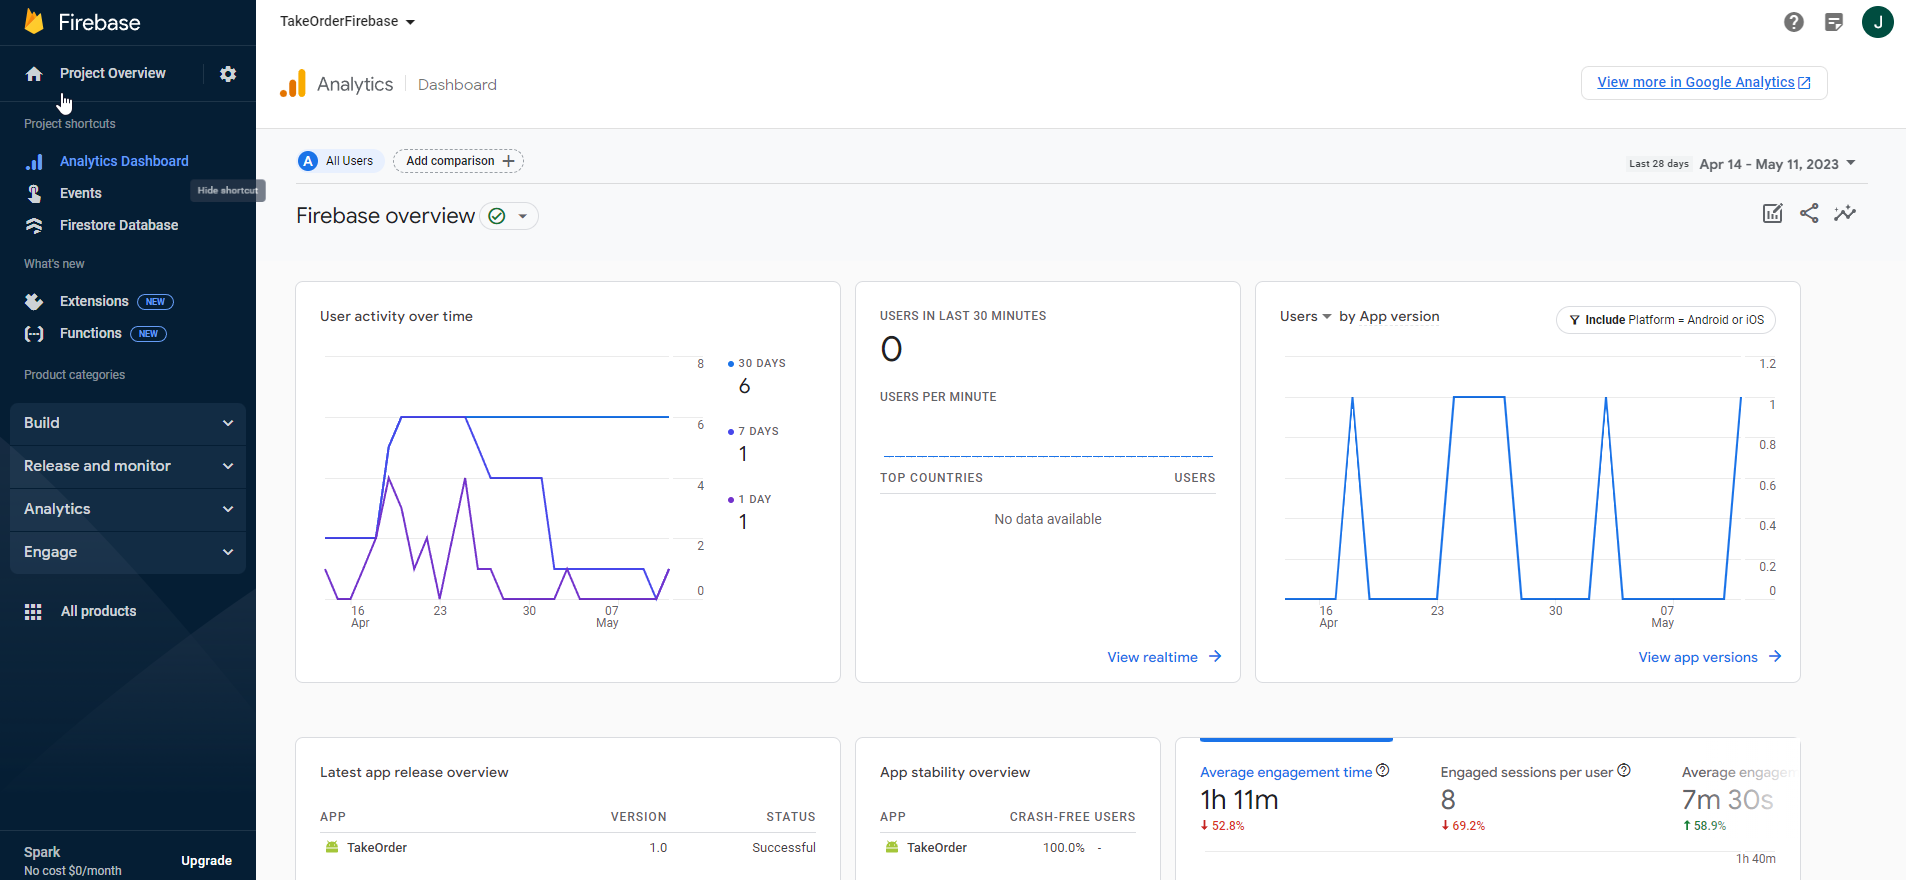
\includegraphics[width=13cm, height=7cm]{Imagenes/Figuras/analyticsFirestore} 
   \caption{Analíticas de un proyecto Firestore\label{fig:Analytics}}
\end{figure}

\begin{figure}[h]
    \centering
    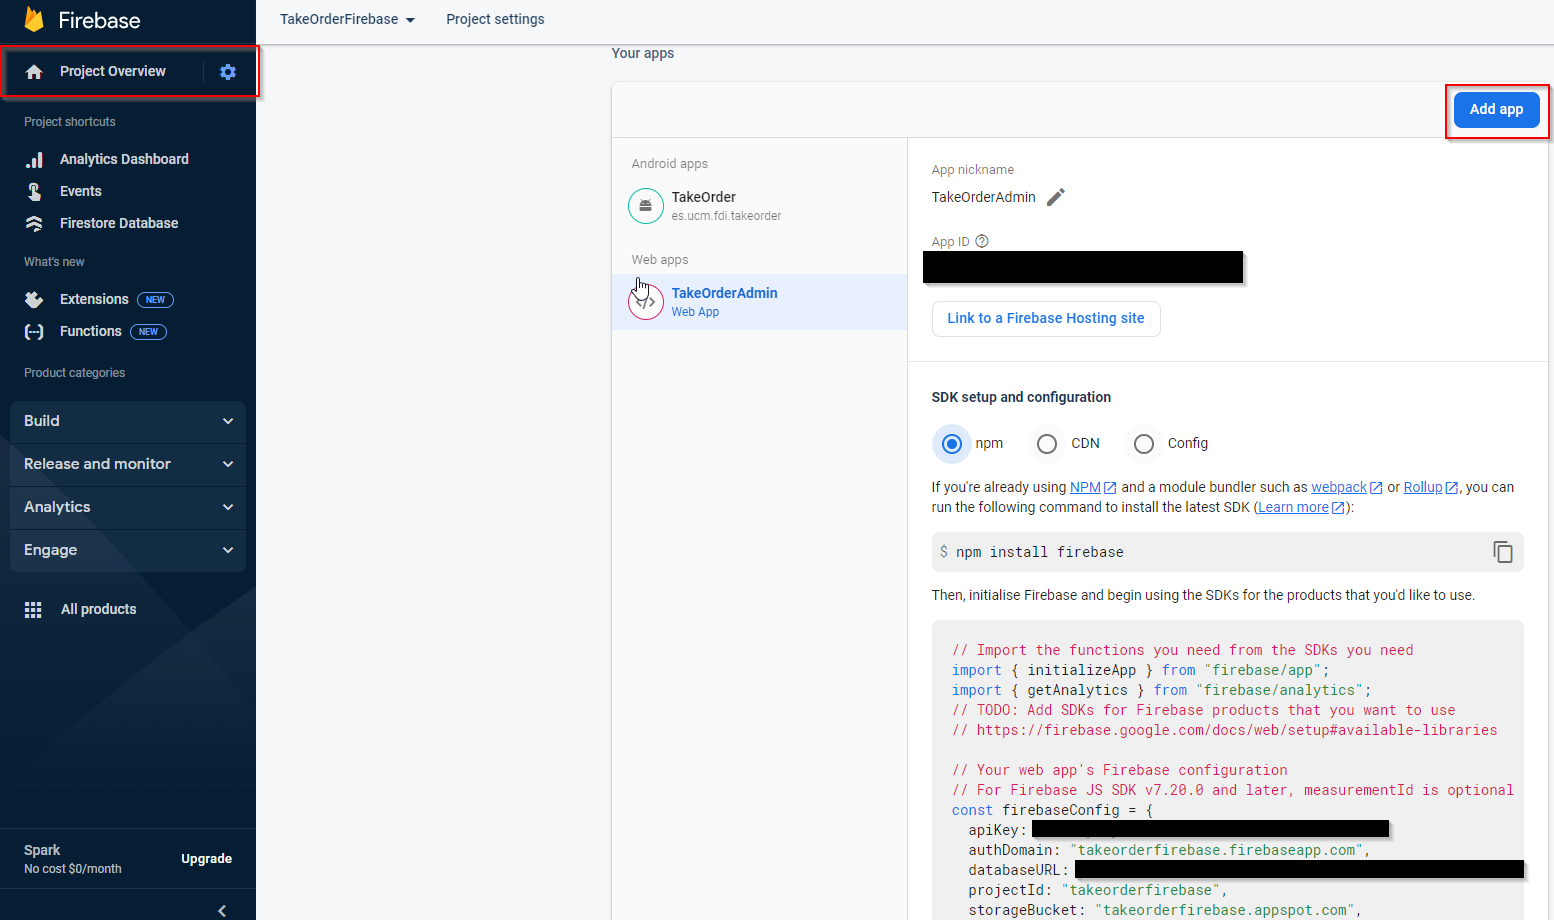
\includegraphics[width=13cm, height=7cm]{Imagenes/Figuras/addAppFirestore.png} 
   \caption{Vincular el proyecto de Firestore a las aplicaciones\label{fig:AddApp}}
\end{figure}

\section{Despliegue de la página web}


Las aplicaciones web se ejecutan en un servidor. En nuestro proyecto se utiliza para el \textit{back-end} la plataforma que nos ofrece Fly.io, y para el \textit{front-end}, \textit{Firebase}.

Fly.io es un \textit{PaaS} (\textit{Platform as a service}) que nos permite manejar el servidor y sus configuraciones. Su
arquitectura es mucho más robusta y segura que un \textit{hosting}.

El proceso para el despliegue ha consistido en registrarnos en Fly.io, y desplegar nuestra aplicación. Fly.io te ofrece distintas maneras para desplegar tu aplicación: desde diferentes \textit{frameworks} web (Django, Phoenix, Rails...) seleccionando un lenguaje de programación (Ruby, Python....) hasta despliegue con un \textit{Dockerfile}.
Como nuestra aplicación no usaba ningún \textit{framework} de las opciones que nos daba Fly.io, decidimos crear un \textit{dockerfile} para nuestra aplicación.

\subsection{Docker}

Para poder desplegar nuestra aplicación en Fly.io necesitamos tener un \textit{Dockerfile} o una imagen de nuestro proyecto.
Un \textit{Dockerfile} es un archivo de texto que contiene las instrucciones necesarias para crear una nueva imagen.
Una imagen de \textit{Dcoker} es una plantilla de solo lectura que define su contenedor. La imagen contiene el código que se ejecutará, incluida cualquier definición para cualquier biblioteca o dependencia que el código necesite.

Para conseguir esa imagen utilizamos un \textit{plugin} de Google: \textit{jib-maven-plugin}.
Para construir la imagen usamos el comando \texttt{mvn compile jib:dockerBuild} desde la terminal de VSCode. Ahora tenemos la imagen \textit{docker} creada, y podemos visualizarla desde la aplcación de escritorio de \textit{Docker} (Figura~\ref{fig:DockerDesktop}).

\begin{figure}[h]
    \centering
    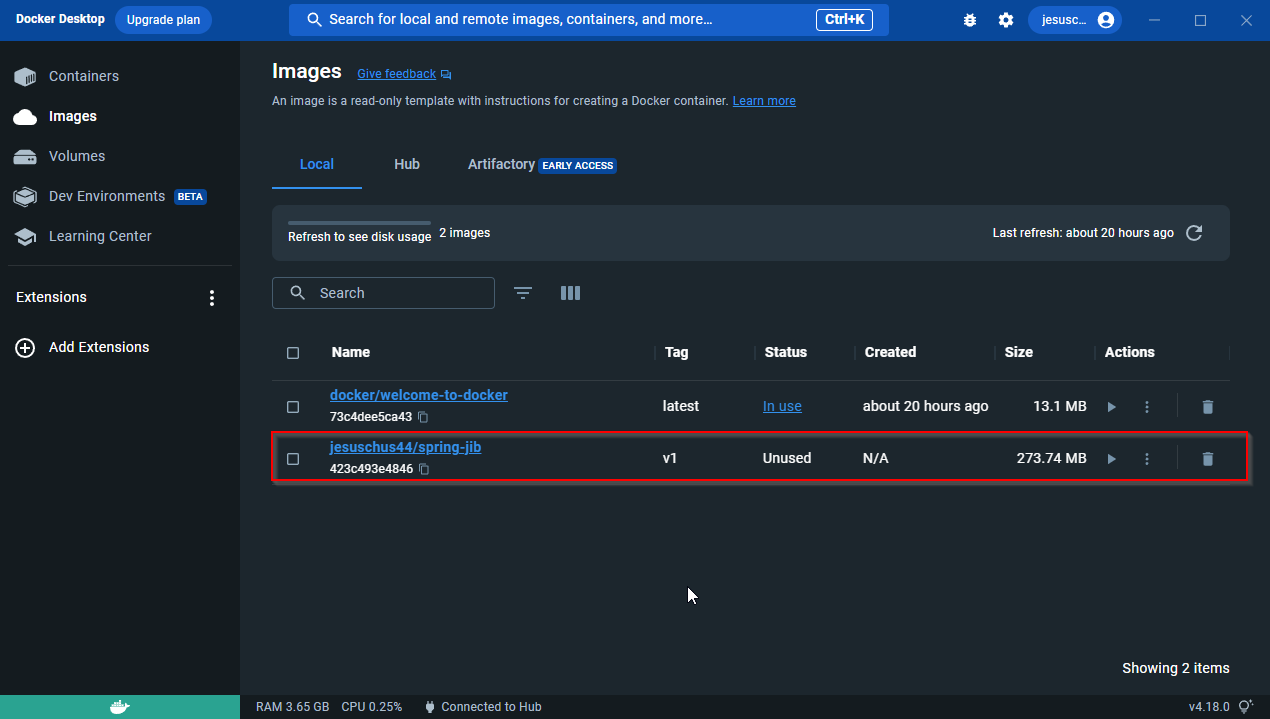
\includegraphics[width=14cm, height=8cm]{Imagenes/Figuras/docker desktop.png} 
   \caption{Aplicación de escritorio Docker Desktop\label{fig:DockerDesktop}}
\end{figure}

Para poder usar esa imagen en Fly.io tenemos que publicarla en \textit{Docker hub}, que es un repositorio público de imágenes.
Para hacer esto tenemos que ejecutar una serie de comandos desde el \textit{Powershell} de Windows:

\begin{itemize}
\item Hacemos login en nuestra cuenta de \textit{Docker}.
\item Se prepara la imagen para que sea aceptada en este registro público. Todos los registros siguen una nomenclatura a la hora de almacenar los repositorios. En el caso de \textit{Docker hub} necesitamos que nuestra imagen se llame \texttt{nombredeusuario/nombredelrepositorio:etiqueta}. En nuestro caso, \texttt{jesuschus44/spring-jib:v1}.
\item Por último, usaremos el comando \texttt{docker push jesuschus44/spring-jib:v1} para publicar nuestra imagen en el \textit{Docker hub}.
\end{itemize}


\subsection{Despliegue en Fly.io}

Ahora sí, con nuestra imagen publicada en nuestro repositorio de \textit{Docker}, podemos desplegar nuestra aplicación en Fly.io. mediante los siguientes comandos:

\begin{itemize}
\item Primero instalaremos \textit{flyctl}: 
\begin{center}
    \texttt{powershell -Command iwr https://fly.io/install.ps1 -useb | iex}
\end{center}

\item Después nos \textit{logueamos} en fly.io: \texttt{fly auth login}
\item Por último, lanzamos nuestra aplicación: 

\begin{center}
    \texttt{fly launch - -image jesuschus44/spring-jib:v1} 

\end{center}

\begin{figure}[h]
    \centering
    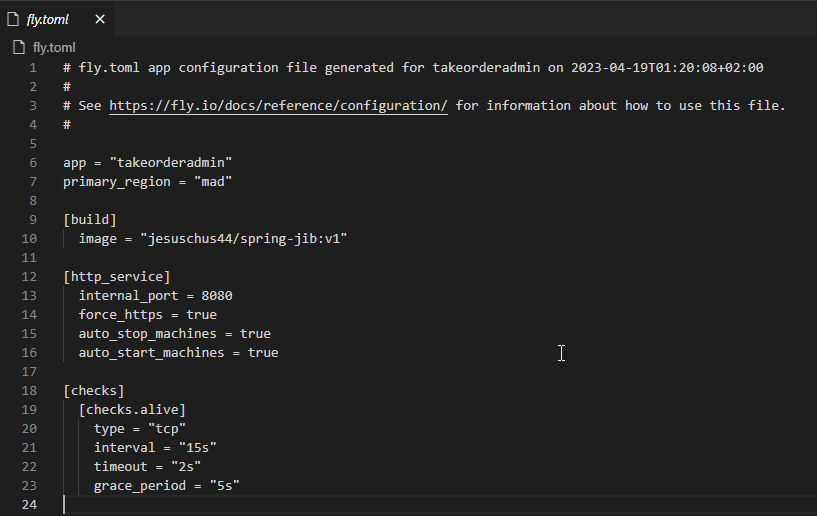
\includegraphics[width=14cm, height=8cm]{Imagenes/Figuras/fly.toml.png} 
   \caption{Archivo fly.toml\label{fig:flytoml}}
\end{figure}

Cada aplicación Fly.io necesita un archivo fly.toml (Figura~\ref{fig:flytoml}) para indicar al sistema como desplegarla. El archivo fly.toml se puede generar automáticamente con el comando \texttt{fly launch}, que nos hará algunas preguntas para configurar todo.
Nos preguntará por un nombre para nuestra aplicación, una región y si queremos una base de datos \textit{Postgres o Redis}. Finalmente, nos pregunta si queremos desplegar para lo que usará la configuración que ha creado en el archivo fly.toml.
Ahora ya podemos visitar nuestra web. La dirección será el nombre de nuestra aplicación.fly.dev, en nuestro caso \url{https://takeorderadmin.fly.dev/}
\end{itemize}



\section{Fase de Desarrollo}
En esta sección se muestra como hemos generado las distintas vistas para la aplicación móvil y para la aplicación web. En cada uno de los apartados describiremos cada una de las funcionalidades de cada vista.

\subsection{Aplicación Móvil}

\subsubsection*{Lista de mesas asignadas}

En esta vista el usuario, como se aprecia en la Figura~\ref{fig:mesaAsignada}, podrá observar el listado de mesas asignadas en el restaurante. 

\begin{itemize} 

\item El botón flotante, de color verde azulado, nos permite generar una nueva ventana en la que podremos añadir una nueva mesa.
 
\item El botón \textit{editar}, asociado a cada mesa, nos generará una nueva ventana en la que se permitirá modificar los datos de la mesa seleccionada.
 
 \item El botón \textit{comanda}, asociado a cada reserva, nos genera una nueva ventana, en la que se permitirá crear una comanda para la mesa seleccionada.
 
 \item El botón \textit{eliminar}, asociado a cada mesa, borrara la misma, y la eliminará del listado de mesas asignadas.
 
 \end{itemize}

 \begin{figure}[h]
 \centering
  \subfloat[Lista de mesas asignadas]{\label{fig:mesaAsignada}
    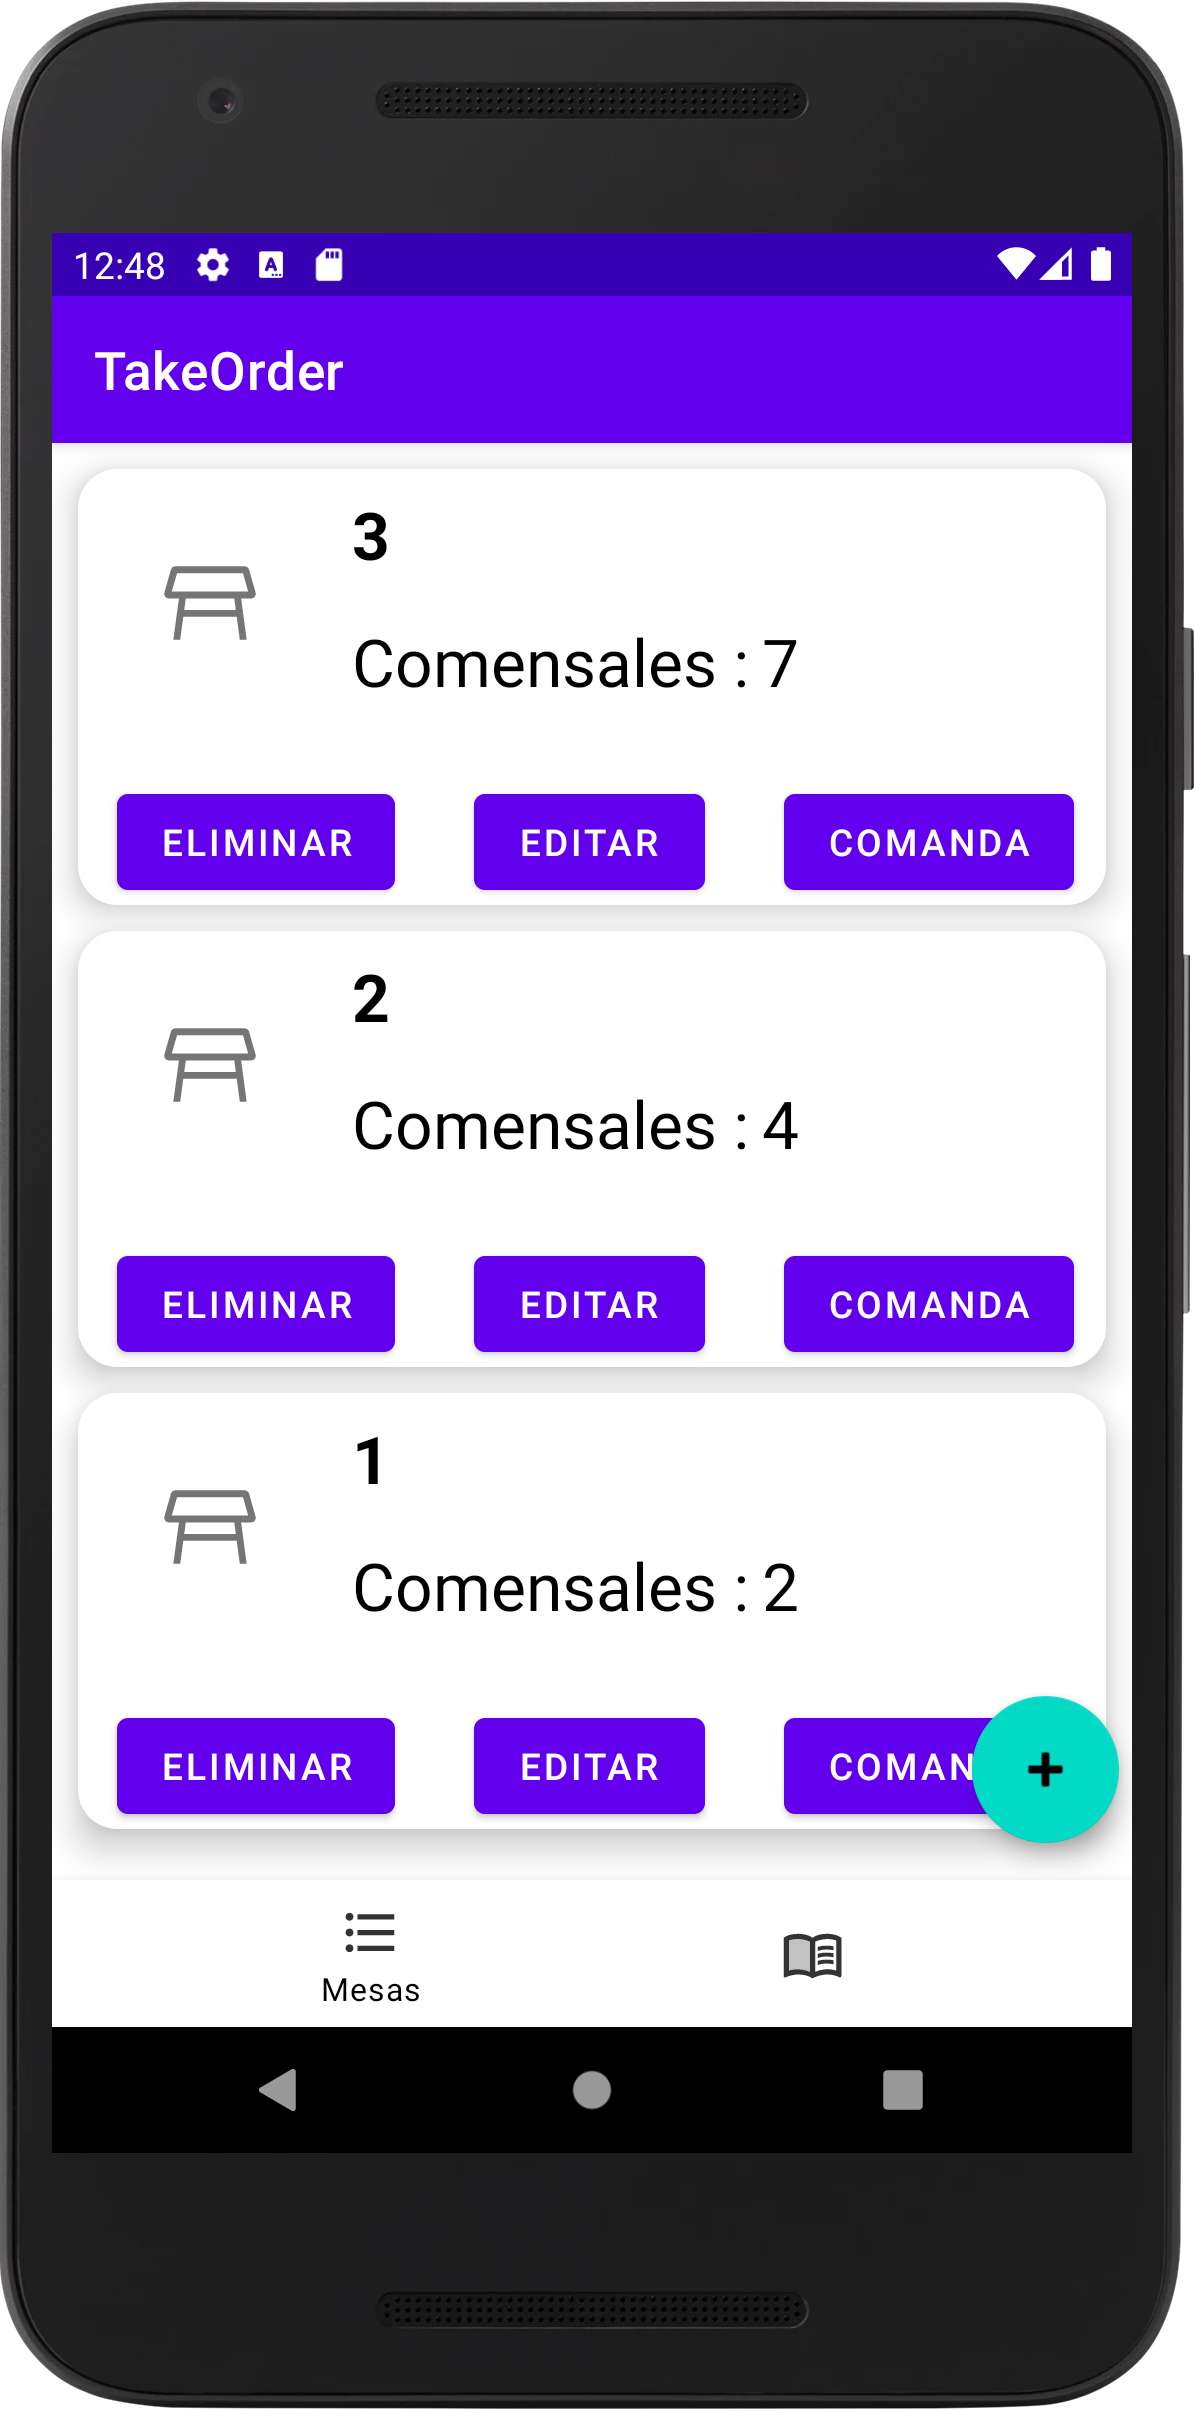
\includegraphics[width=4cm, height=8cm]{Imagenes/Figuras/ListadoMesas.png}}
    \hfill
  \subfloat[Añadir una nueva mesa]{\label{fig:añadirMesa}
   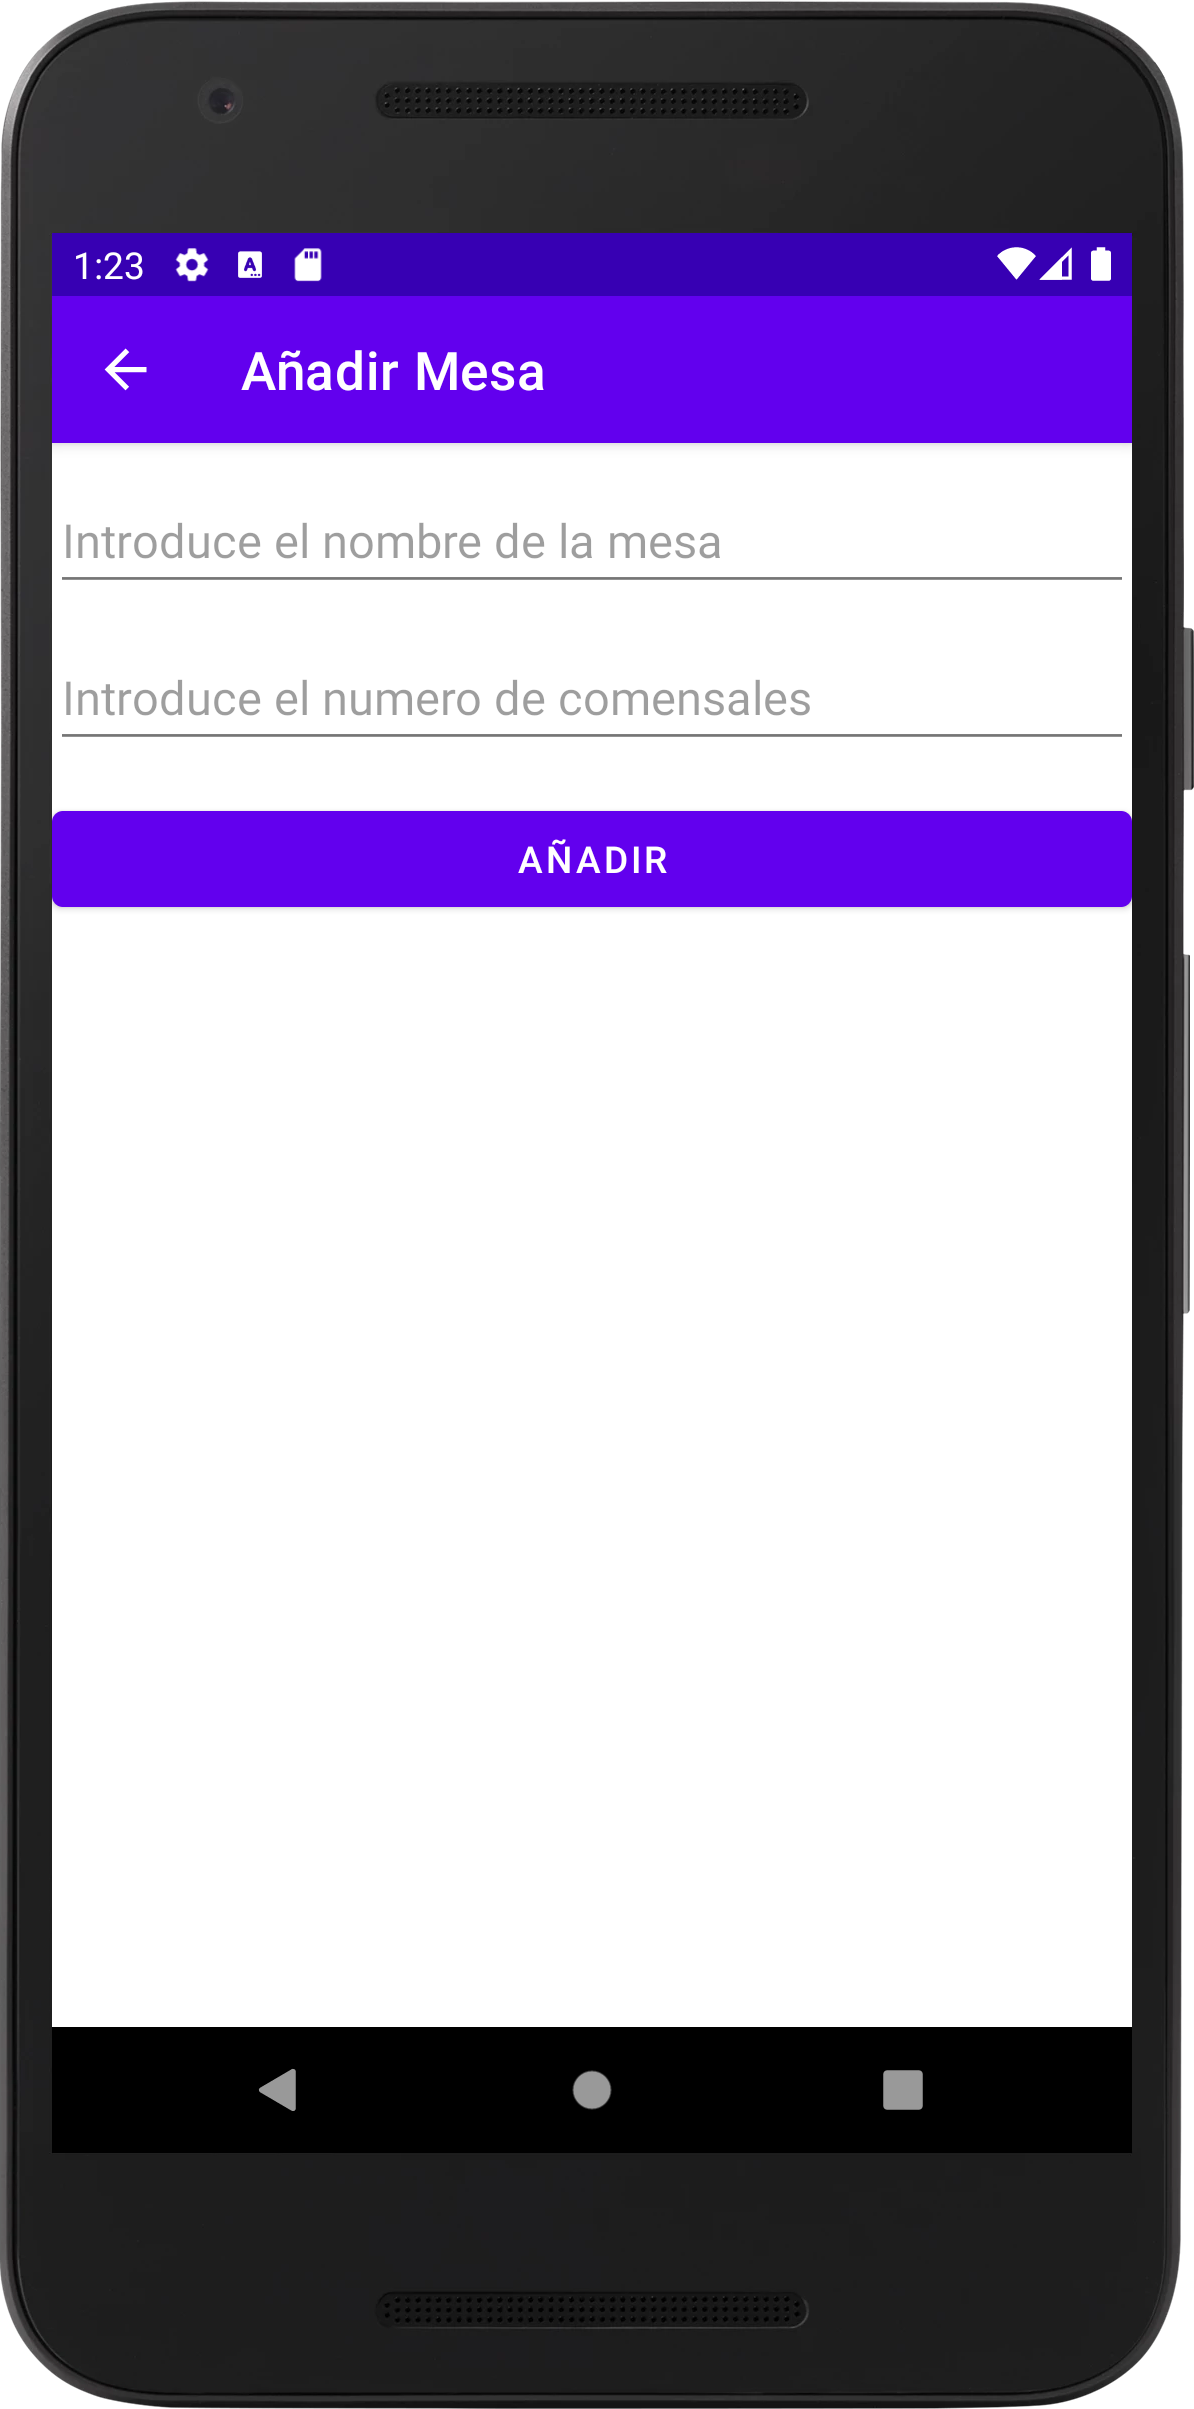
\includegraphics[width=4cm, height=8cm]{Imagenes/Figuras/AñadirMesa.png}}
 \caption{Añadir mesa en aplicación móvil y Lista de mesas asignadas}
\label{fig:ListaMesaYAñadirMesa}
\end{figure}

 
 
 \subsubsection*{Añadir una nueva mesa}
 En esta vista el usuario, como se aprecia en la Figura~\ref{fig:añadirMesa}, accederá a la ventana para añadir una nueva mesa. 

\begin{itemize} 

\item El primer campo nos permitirá introducir el identificador de la mesa que asignaremos.
 
 \item El segundo campo nos permitirá introducir el número de comensales.
 
\item El botón \textit{añadir} validará los datos y añadirá la nueva mesa asignada.
 
\end{itemize}


 \subsubsection*{Editar una mesa asignada}
 En esta vista el usuario, como se aprecia en la Figura~\ref{fig:editarMesa}, podrá editar una mesa ya asignada.

 \begin{itemize} 

\item El primer campo permitirá modificar el nombre de la mesa asignada.
 
 \item El segundo campo permitirá modificar el número de comensales.
 
\item El botón \textit{actualizar} validará los datos y modificará la mesa asignada.
 
\end{itemize}
 

\subsubsection*{Generar nueva comanda a una mesa asignada}
 En esta vista, el usuario, como se aprecia en la Figura~\ref{fig:generarComanda}, podrá seleccionar que tipo de comanda desea el cliente.

 
 \begin{itemize} 

\item El botón \textit{carta}, nos generará una nueva ventana en la que se permitirá generar una comanda pudiendo seleccionar productos de la carta.
 
\item El botón \textit{menú}, nos generará una nueva ventana en la que se permitirá generar una comanda pudiendo seleccionar los platos del menú diario.

\end{itemize}

\begin{figure}[h]
 \centering
   \subfloat[Editar una mesa]{\label{fig:editarMesa}
    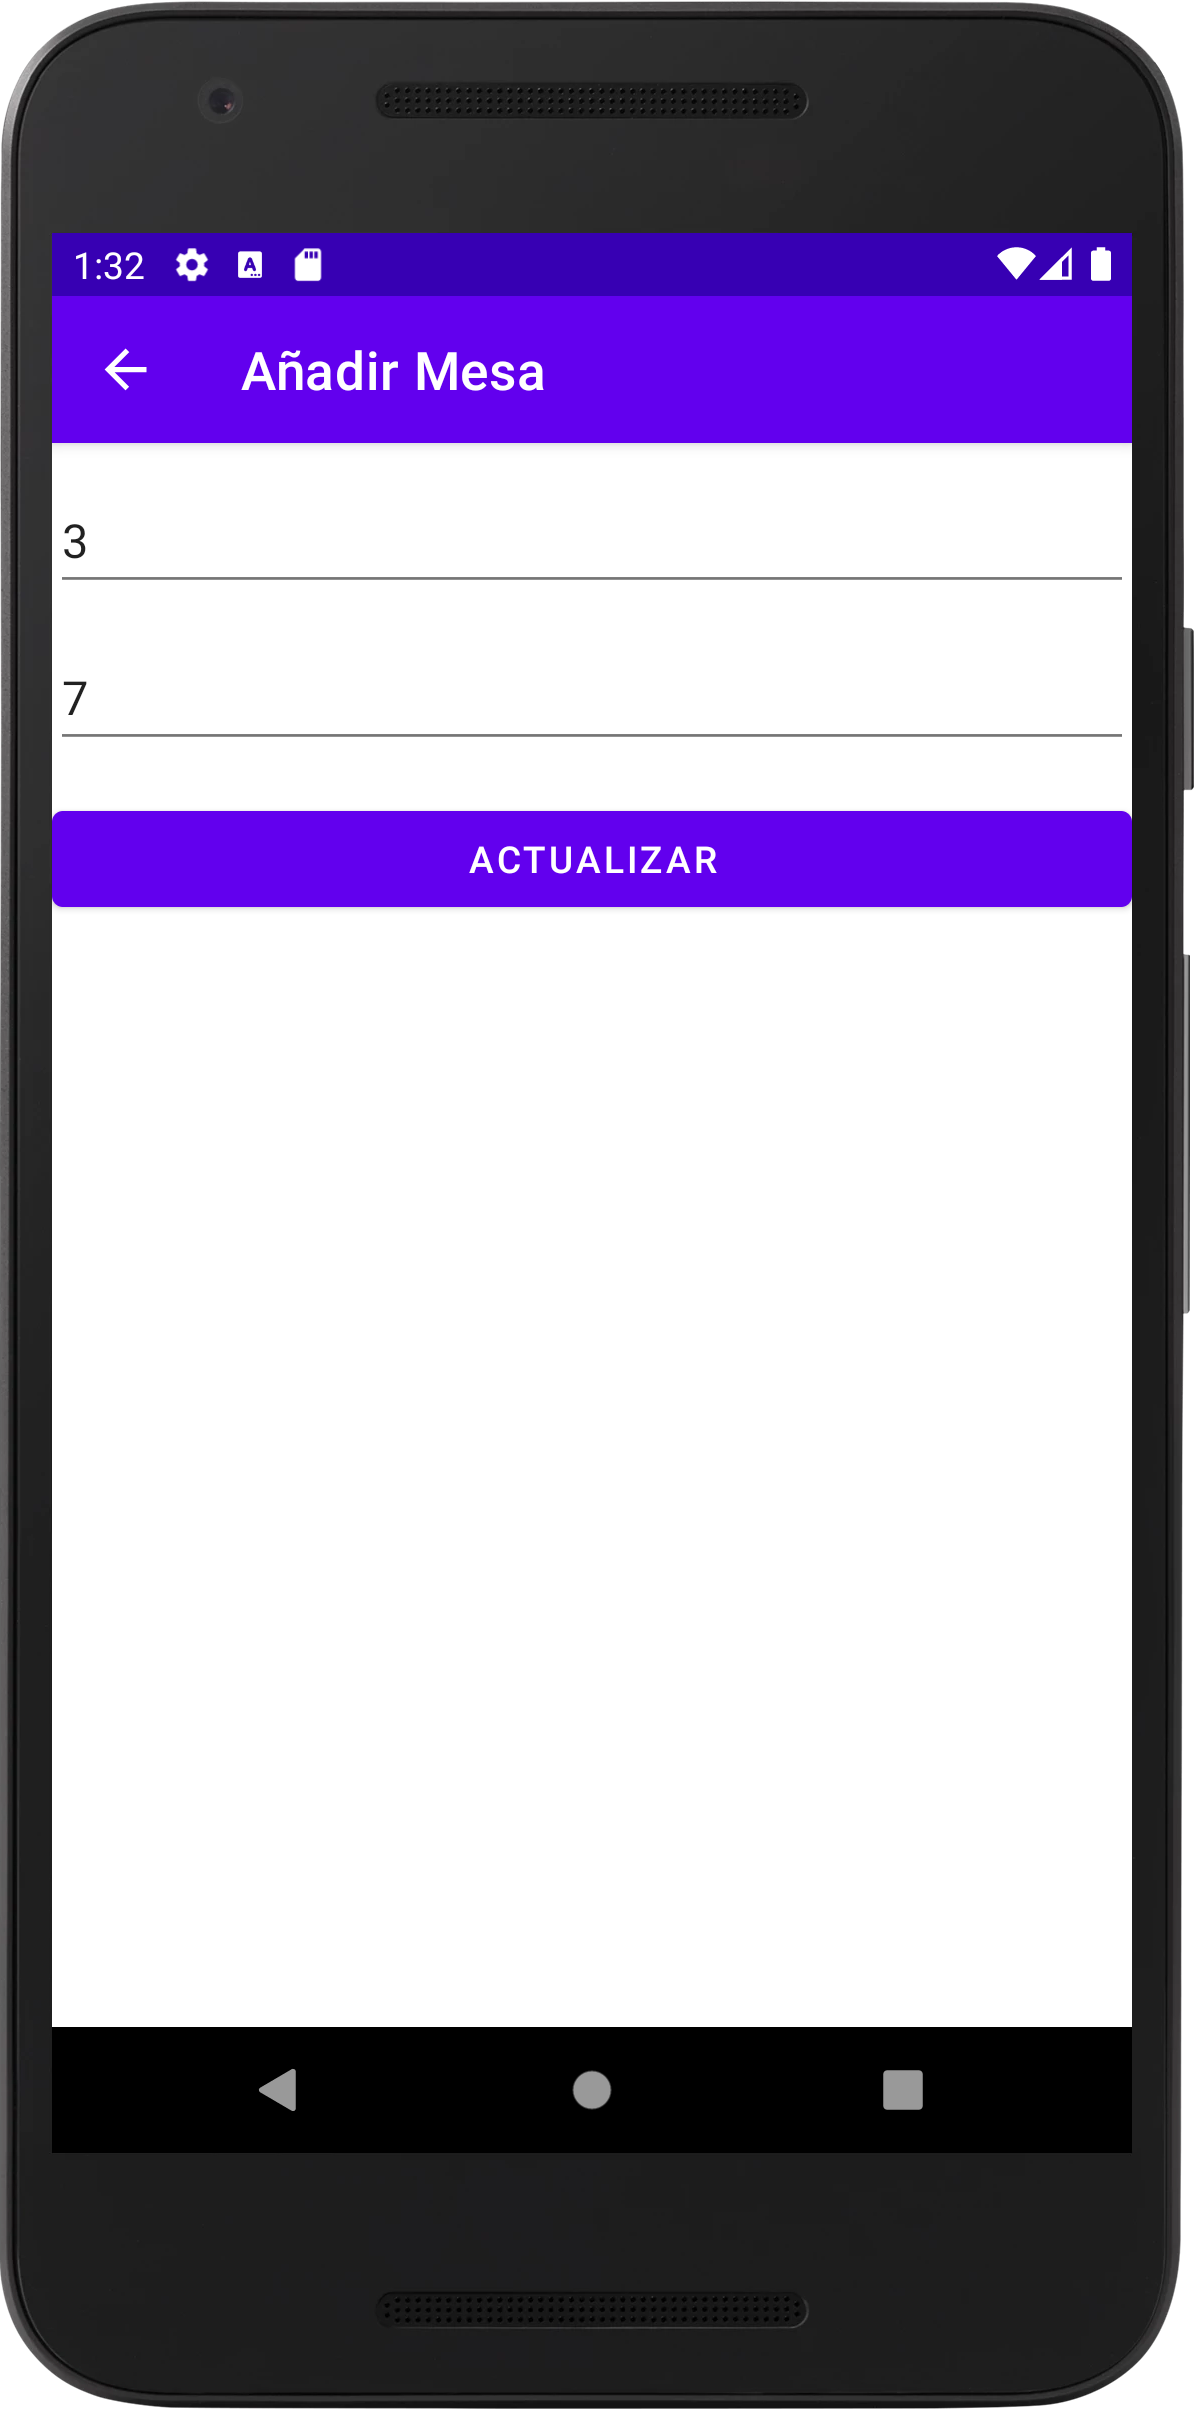
\includegraphics[width=4cm, height=8cm]{Imagenes/Figuras/EditarMesa.png}}
     \hfill
  \subfloat[Generar una comanda]{\label{fig:generarComanda}
   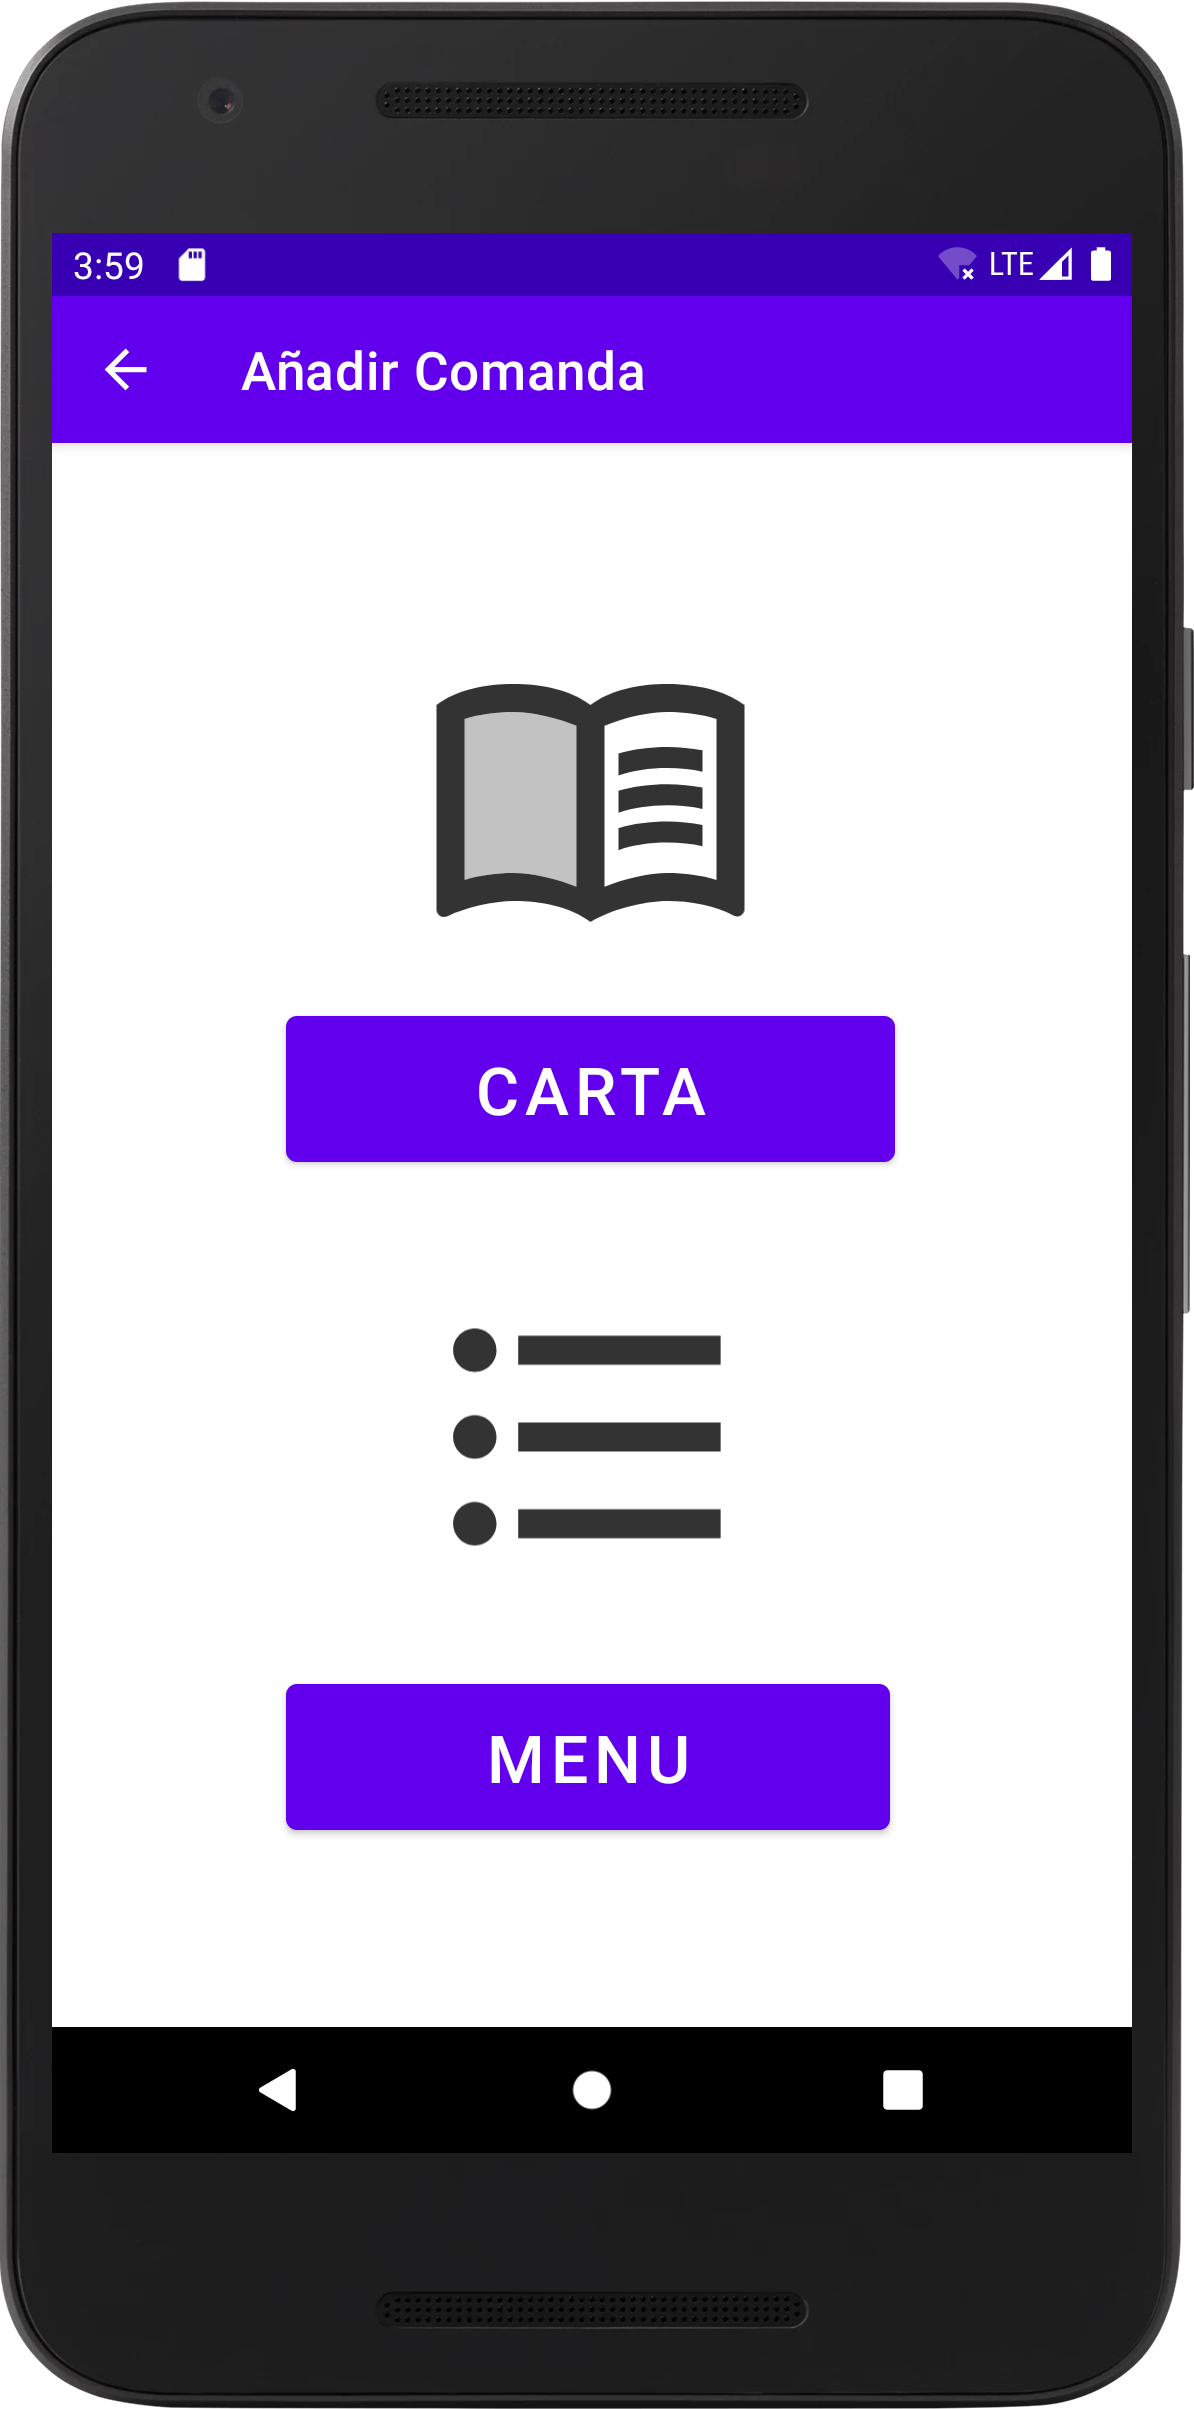
\includegraphics[width=4cm, height=8cm]{Imagenes/Figuras/MenuOCarta.png}}
 \caption{Generar comanda y editar mesa}
\label{fig:GenerarComandaYEditarMesa}
\end{figure}

\subsubsection*{Carta}
 En esta vista, el usuario, como se aprecia en la Figura~\ref{fig:verCarta}, podrá añadir los elementos de la carta deseados, además de poder ver el listado de los elementos solicitados.
 
 \begin{itemize} 

\item El botón \textit{añadir bebidas}, nos generará una nueva ventana en la que se listara todas las bebidas disponibles.
 
\item El botón \textit{bebidas pedidas}, nos generará una nueva ventana en la que listara las bebidas pedidas hasta el momento.

\item El botón \textit{añadir platos}, nos mostrará una nueva ventana en la que se listara todos los platos disponibles.
 
\item Por último, el botón \textit{platos pedidos}, nos llevará a una nueva ventana en la que se listarán los platos pedidos hasta el momento.
\end{itemize}


\subsubsection*{Añadir bebidas}
 En esta vista el usuario, como se aprecia en la Figura~\ref{fig:añadirBebidasCarta}, podrá ver el listado de las bebidas disponibles, pudiendo añadir la bebida y la cantidad deseadas.
 
 \begin{itemize} 

\item El primer campo nos permitirá introducir el número de bebidas que deseamos añadir, debiendo ser menor que la cantidad total disponible.

\item El botón \textit{añadir}, nos generará una nueva ventana de confirmación en la que nos mostrará la cantidad introducida, y el nombre de la bebida que deseamos añadir, pudiendo seleccionar el botón \textit{cancelar} o \textit{aceptar} para confirmar el pedido.


\end{itemize}

\begin{figure}[h]
 \centering
   \subfloat[Elementos de la Carta]{\label{fig:verCarta}
    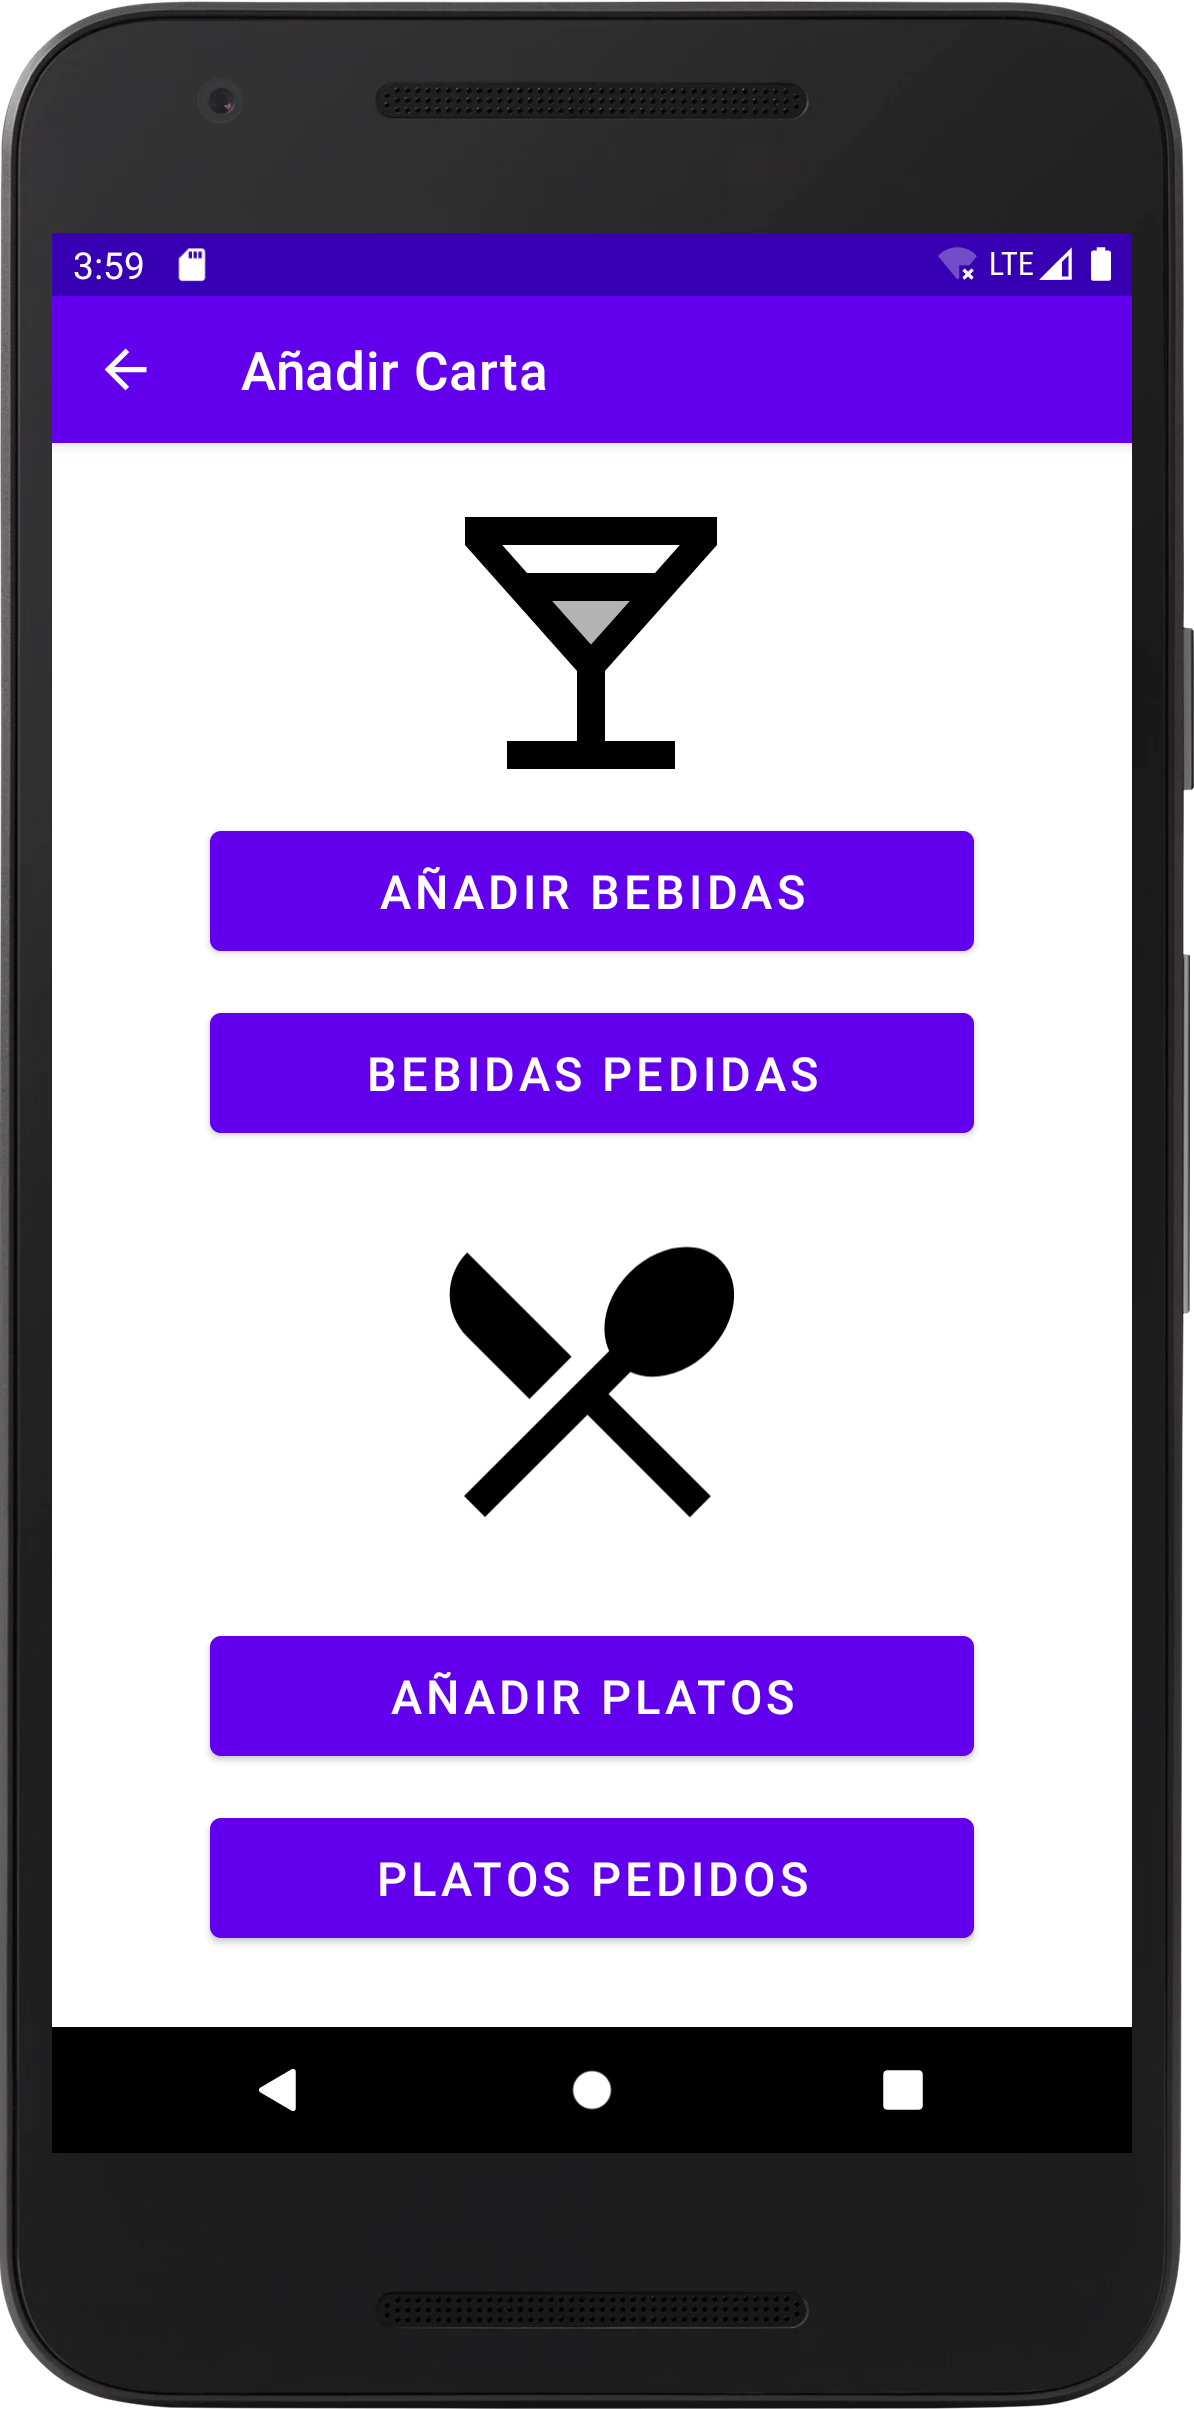
\includegraphics[width=4cm, height=8cm]{Imagenes/Figuras/VerCarta.png}}
    \hfill
    \subfloat[Añadir bebidas]{\label{fig:añadirBebidasCarta}
   \includegraphics[width=4cm, height=8cm]{Imagenes/Figuras/AñadirBebidasCarta.png}}
 
 \caption{Añadir bebidas y ver carta}
\label{fig:AñadirBebidasYVerCarta}
\end{figure}



\subsubsection*{Lista de bebidas pedidas}
 En esta vista, el usuario podrá ver el listado de las bebidas pedidas Figura~\ref{fig:listaBebidasPedidas} con la cantidad pedida de cada bebida .
 
 \begin{itemize} 

\item El botón \textit{pendiente} estará seleccionado por defecto cuando se añada una nueva bebida y permanecerá en ese estado hasta que se haga entrega de las bebidas a la mesa. El botón \textit{pendiente} se deshabilitará cuando se seleccione el botón entregado.

\item El botón \textit{entregado} estará sin seleccionar por defecto cuando se añada una nueva bebida, cuando se haga entrega de las bebidas en la mesa el usuario podrá seleccionar el botón \textit{entregado}.
\end{itemize}

\begin{figure}[h]
    \centering
    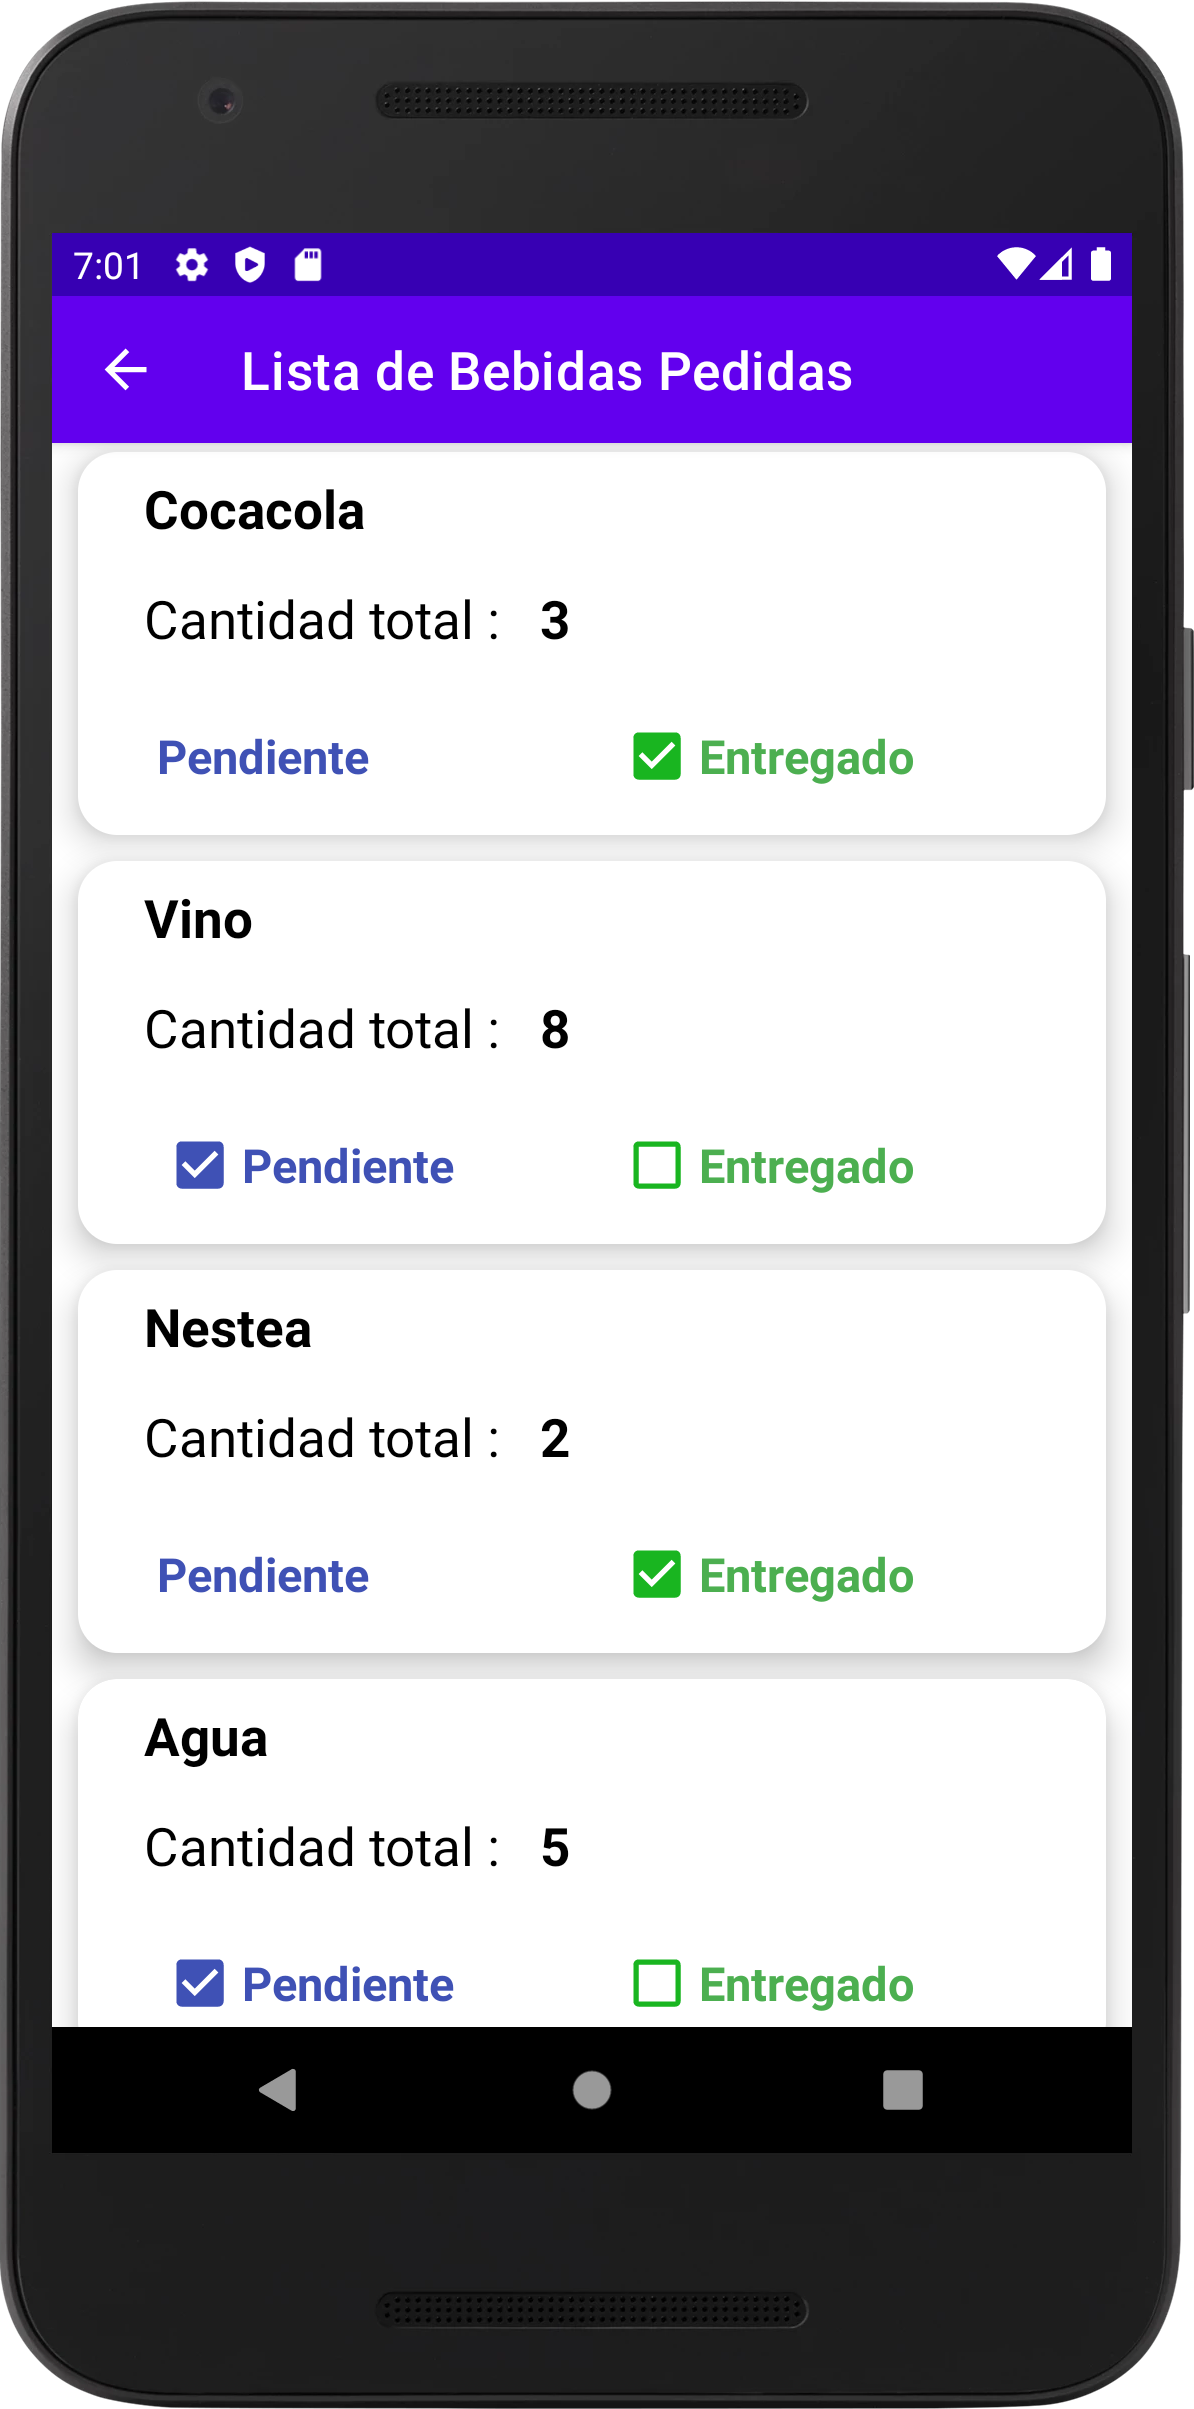
\includegraphics[width=4cm, height=8cm]{Imagenes/Figuras/ListaBebidasPedidas.png}
   \caption{Lista de bebidas pedidas
    \label{fig:listaBebidasPedidas}}
\end{figure}


\subsection{Aplicación Web}

\subsubsection*{Listado de ingredientes}
Esta vista contiene el listado de todos los ingredientes del restaurante. Por defecto, la tabla está ordenada por el nombre de los ingredientes como se aprecia en la Figura~\ref{fig:listaingredientes}
\begin{itemize} 

\item El botón \textit{Añadir nuevo ingrediente} nos abrirá un \textit{pop up} donde podemos seleccionar todos los valores y datos del ingrediente: nombre, categoría, cantidad, alerta y medida. 

\item También dispone de un filtro y un buscador. El filtro te selecciona los ingredientes de la categoría que selecciones. El buscador, en cambio, busca en la tabla por el nombre del ingrediente.

\item Cada ingrediente dispone de dos botones: editar y eliminar. El botón editar nos muestra un \textit{pop up}, igual que el de añadir ingrediente, pero con los datos rellenos del ingrediente seleccionado, para poder cambiar los campos que nosotros queramos. El botón eliminar abre un \textit{pop up} para eliminar el ingrediente.


\end{itemize}

El objetivo era diseñar una interfaz intuitiva, en la que sea fácil y rápido consultar y gestionar todo el \textit{stock} de ingredientes del restaurante.

\begin{figure}[h]
    \centering
    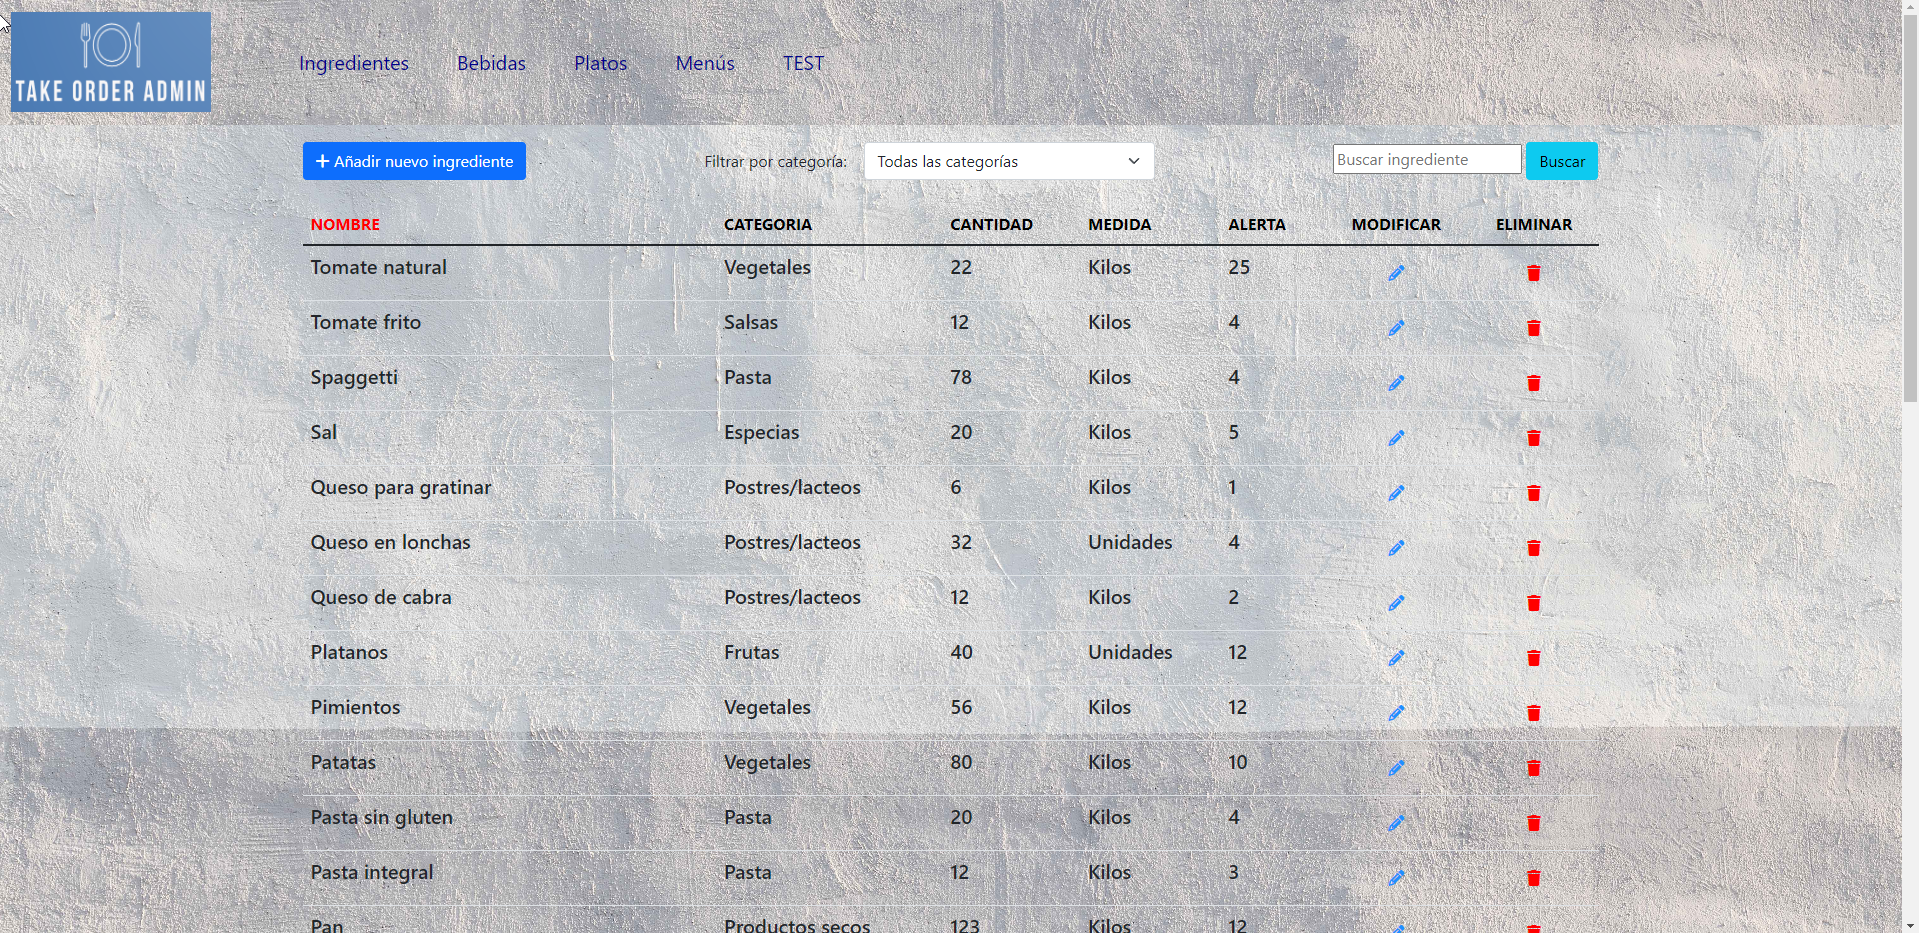
\includegraphics[width=15cm, height=8cm]{Imagenes/Figuras/listaingredientes.png} 
   \caption{Listado de ingredientes\label{fig:listaingredientes}}
\end{figure}

\subsubsection*{Listado de bebidas}

Esta vista nos muestra todas las bebidas disponibles en el restaurante, Figura~\ref{fig:listabebidas}. \begin{itemize} 

\item El botón \textit{Añadir nueva bebida} nos abrirá un \textit{pop up} donde podemos añadir una nueva bebida con sus campos correspondientes: nombre, cantidad y alerta. 

\item En esta ventana solo hay disponible un buscador por nombre de bebida. No hay filtro porque las bebidas no tienen una categoría asociada.

\item Al igual que en la ventana de ingredientes, cada bebida dispone de dos botones: editar y eliminar. El de editar abre un \textit{pop up} con los datos de la bebida donde podemos cambiar el que queramos. El de eliminar, elimina una bebida.


\end{itemize}

\begin{figure}[h]
    \centering
    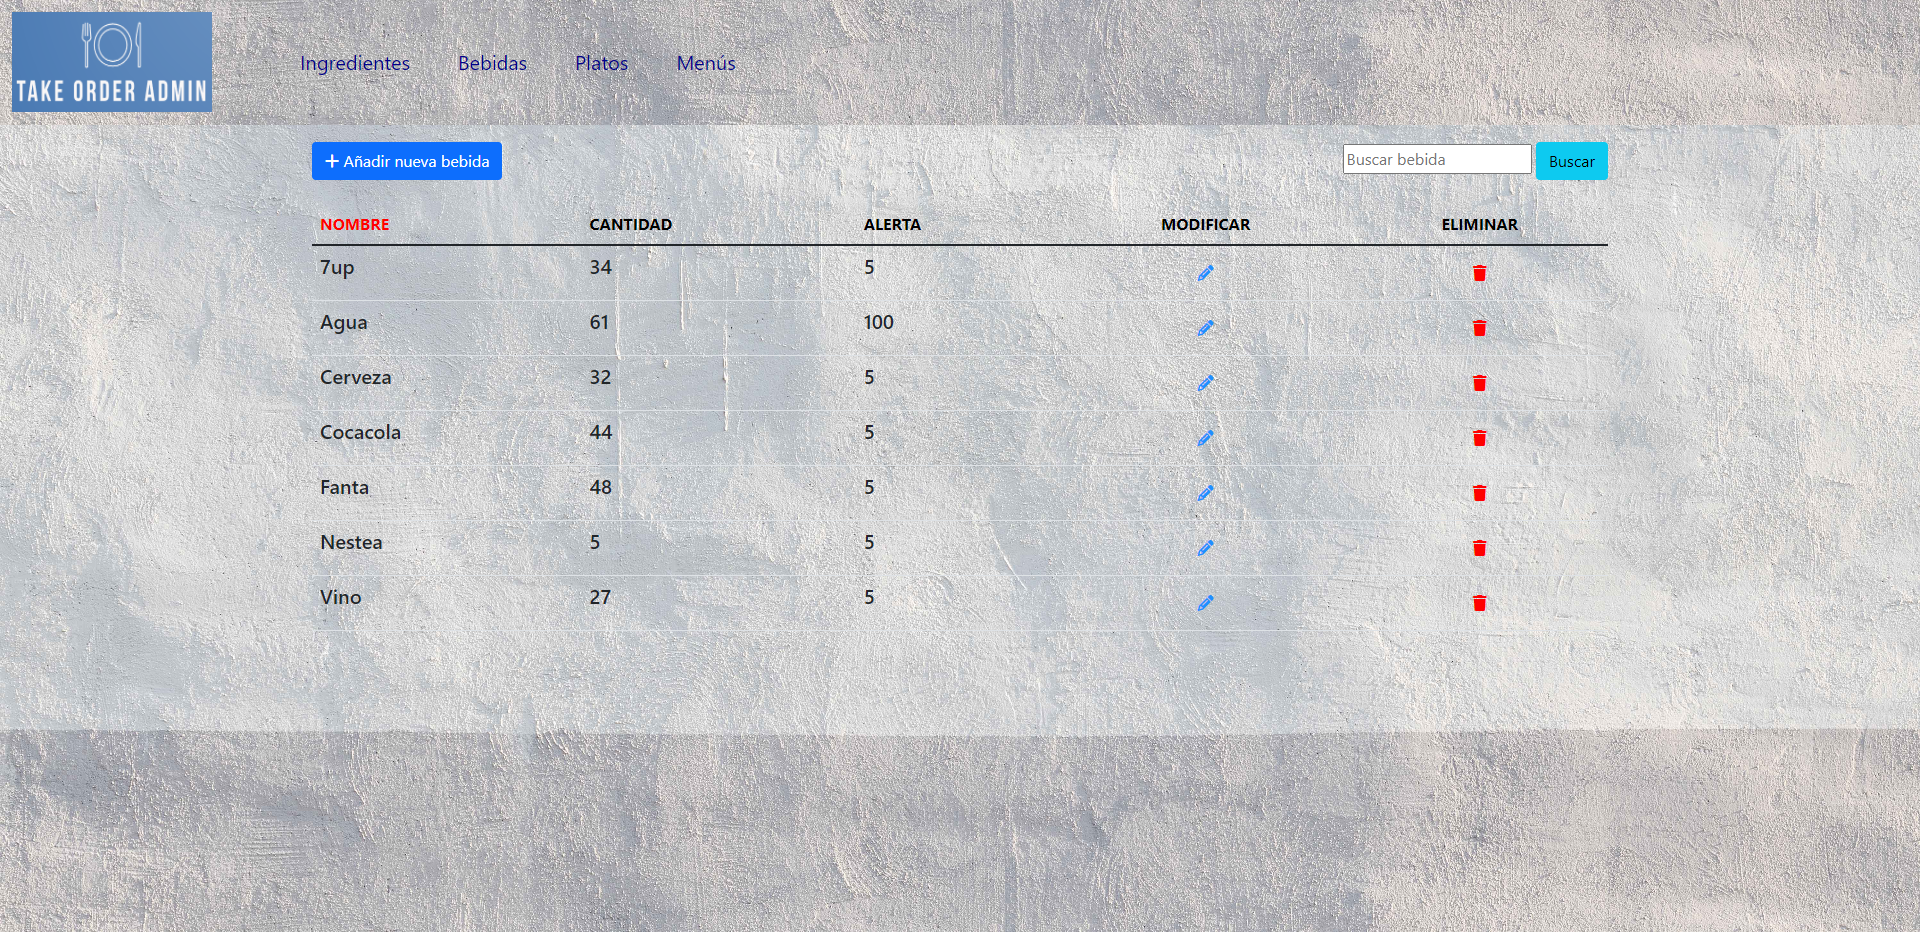
\includegraphics[width=15cm, height=8cm]{Imagenes/Figuras/listabebidas.png} 
   \caption{Listado de bebidas\label{fig:listabebidas}}
\end{figure}

\subsubsection*{Listado de platos}

Aquí mostramos el listado de todos los platos del restaurante, ver Figura~\ref{fig:listaplatos}. 
\begin{itemize} 

\item El botón \textit{Añadir nuevo plato} nos abrirá un \textit{pop up} para añadir un nuevo plato. En el \textit{pop up} deberemos seleccionar un nombre, una categoría y una lista de ingredientes con su cantidad correspondiente. La cantidad es la establecida para una ración de ese plato y cada plato deberá tener al menos un ingrediente. 

\item Dispone de un filtro por categorías (primer plato, bocadillos, postre...) y un buscador global que busca por nombre del plato.

\item Cada plato tiene un botón \textit{Ingredientes} que al pulsar nos muestra un desplegable con los ingredientes y cantidades necesarias para elaborar ese plato.

\item Al igual que los ingredientes y las bebidas, cada plato dispone de dos botones, editar y eliminar, que funcionan igual que los anteriores.

\end{itemize}

\begin{figure}[h]
    \centering
    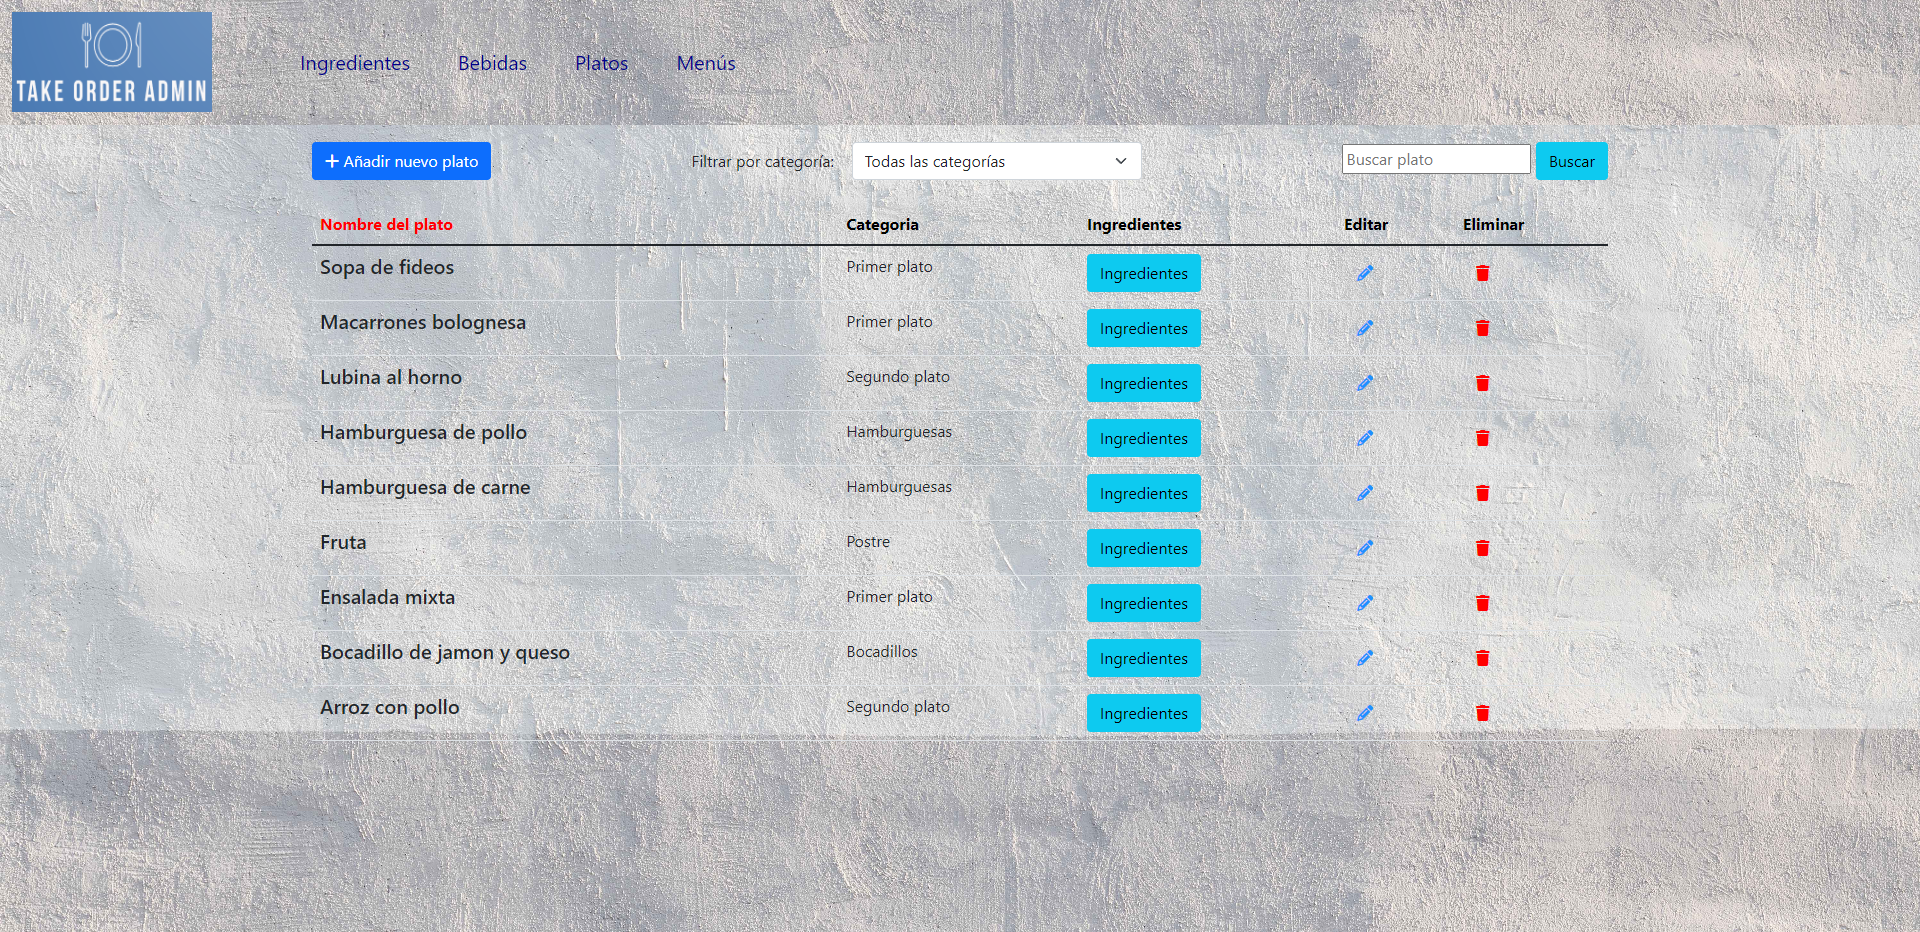
\includegraphics[width=15cm, height=8cm]{Imagenes/Figuras/listaplatos.png} 
   \caption{Listado de platos \label{fig:listaplatos}}
\end{figure}

\subsubsection*{Menú del día}
En la Figura~\ref{fig:menus} podemos ver la vista donde se confecciona el menú diario que servirá el restaurante.

\begin{itemize} 

\item Tiene una tabla donde muestra todos los primeros platos, segundos y postres disponibles, que corresponden a las categorías que compondrán el menú. Cada plato tiene un \textit{checkbox} y una cantidad asociada. Para añadir un plato al menú debemos introducir las raciones que se van a elaborar. Este procedimiento se repetirá con todos los platos que queramos añadir.

\item La tabla de la derecha nos muestra los platos añadidos al menú. Este menú se guarda pulsando el botón \textit{guardar menú}.

\item El botón \textit{guardar menú} se encarga de comprobar que hay disponibilidad de ingredientes para realizar todas las cantidades de los platos que se han añadido al menú. Si no hay suficiente cantidad de algún ingrediente, te lo muestra en un \textit{pop up} para que cambies las cantidades de algún plato o poner otros distintos.

\item En esta vista no se pueden editar los platos ni sus ingredientes, solo se pueden añadir o quitar platos del menú del día.

\end{itemize}

\begin{figure}[h]
    \centering
    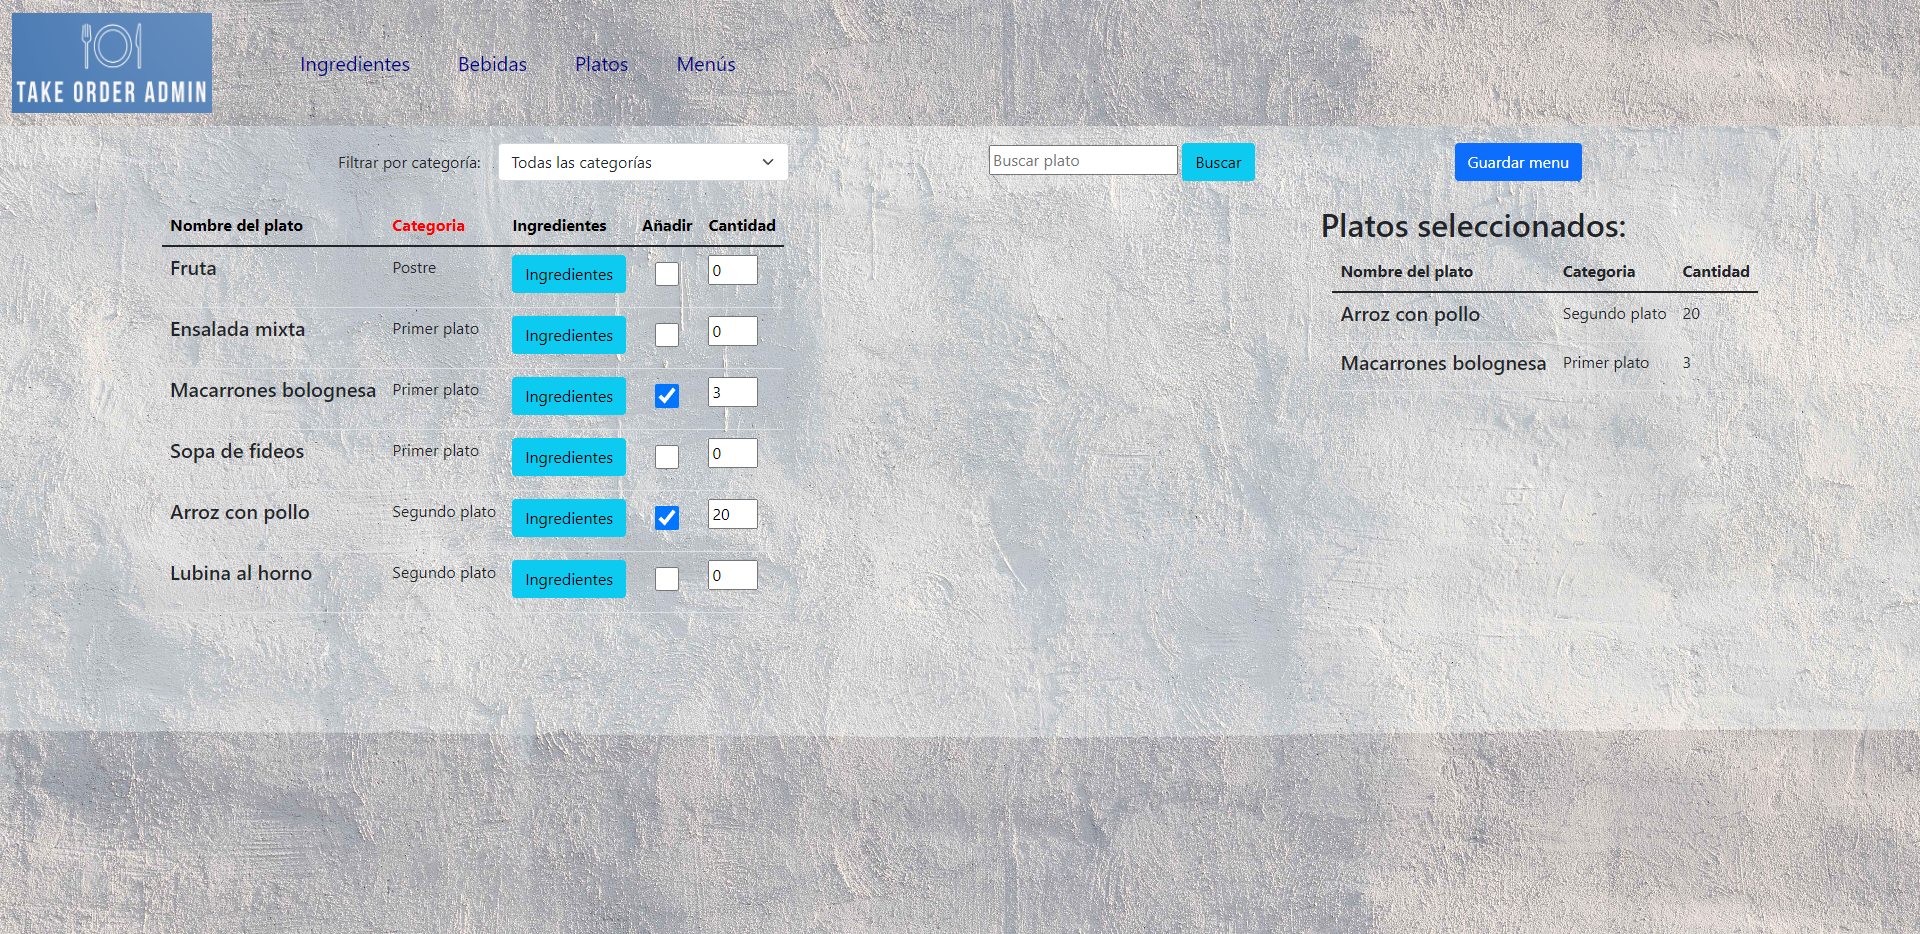
\includegraphics[width=15cm, height=8cm]{Imagenes/Figuras/menus.png} 
   \caption{Menús \label{fig:menus}}
\end{figure}

\subsubsection*{Alertas}
Esta es la página inicial, Figura~\ref{fig:alertas}, donde se muestran los ingredientes y bebidas que tienen un \textit{stock} inferior al nivel de la alerta que se estableció para cada uno de ellos.

\begin{itemize} 

\item Al iniciar la web se muestra un \textit{pop-up} si hay algún ingrediente o bebida bajo de \textit{stock}. 

\item Hay dos tablas, una que muestra las alertas de los ingredientes y otra la de las bebidas. Cada tabla tiene un botón para reponer su stock. Al pulsar en cada botón nos mostrará un \textit{pop-up} para poder reponer el stock de las bebidas o los ingredientes, tanto de los que están por debajo de su alerta y los que no.

\end{itemize}


\begin{figure}[h]
    \centering
    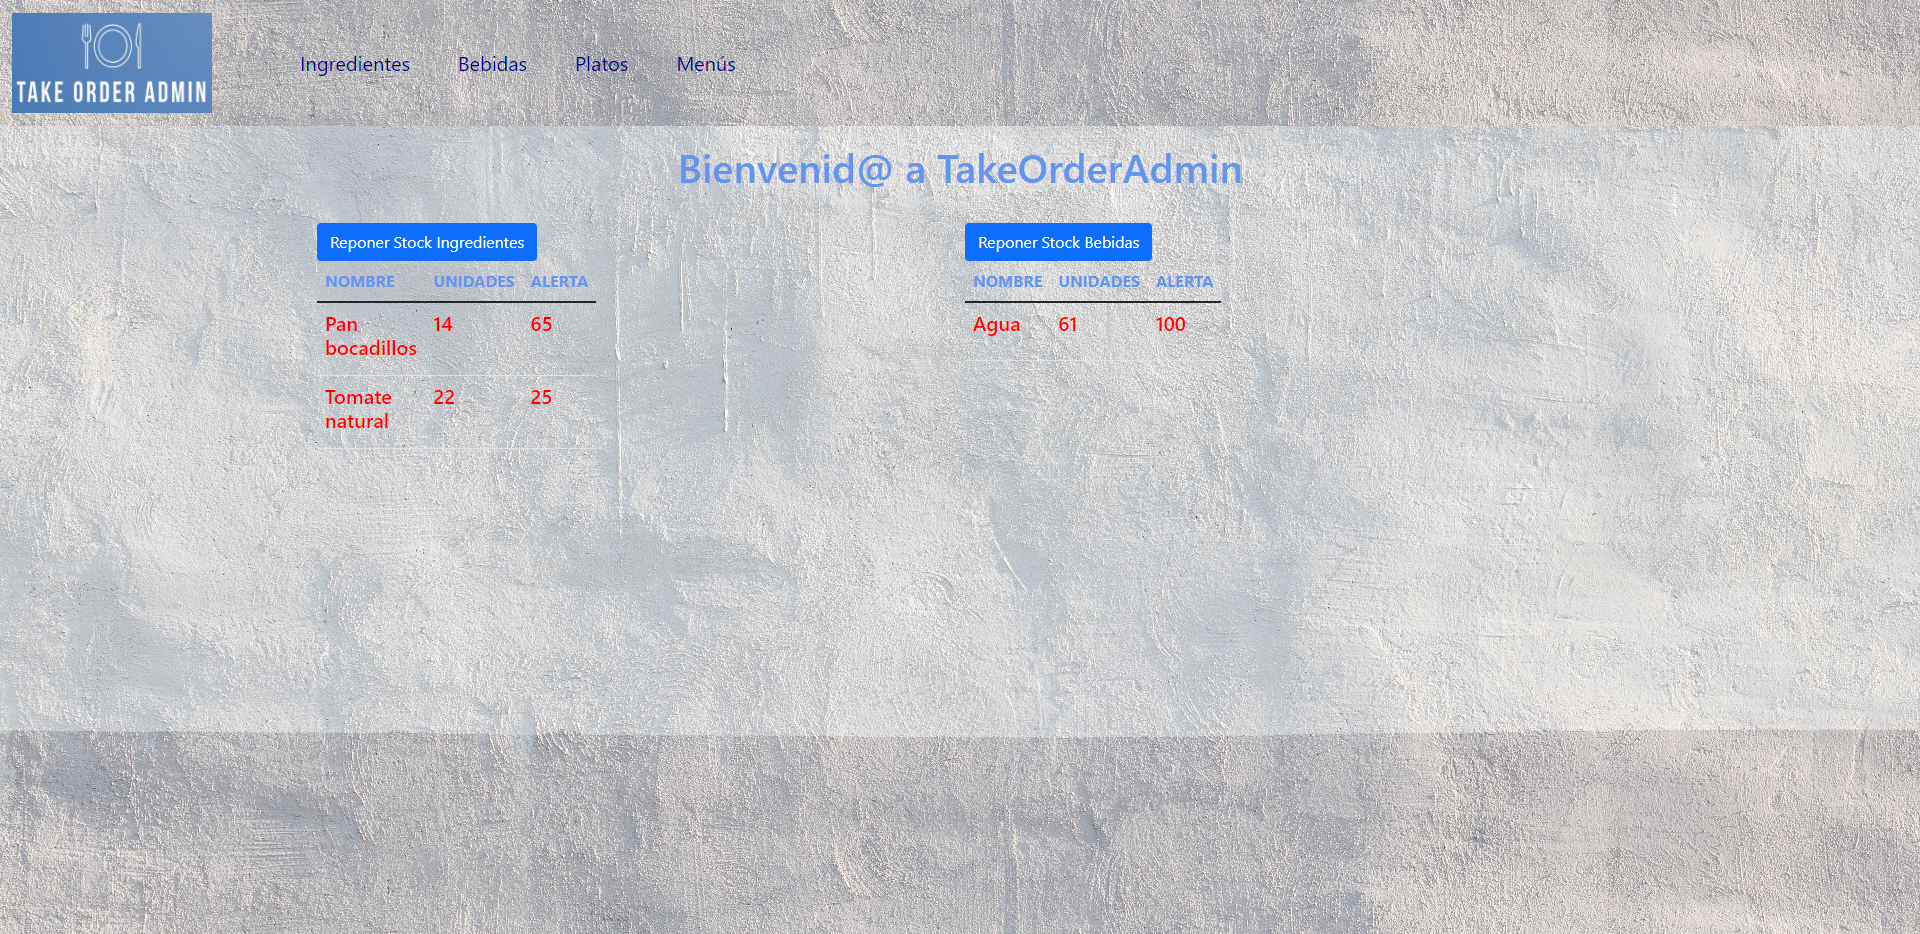
\includegraphics[width=15cm, height=8cm]{Imagenes/Figuras/alertas.png} 
   \caption{Alertas \label{fig:alertas}}
\end{figure}



 


